\documentclass{bmvc2k}
\usepackage[T1]{fontenc}
\usepackage{enumitem}   % for \begin{enumerate}[label=(\arabic*)]
\usepackage{amsmath,amssymb,amsfonts}
\usepackage{graphicx}
\usepackage{algorithm}
\usepackage{algpseudocode}
\usepackage{textcomp}
\usepackage{xcolor}
% \documentclass{article}
\usepackage{booktabs}
\usepackage{multirow}
\usepackage{graphicx}
% \usepackage[margin=1in]{geometry}
\usepackage{hyperref}
\usepackage{multirow}
\usepackage{booktabs}
%% Enter your paper number here for the review copy
% \bmvcreviewcopy{??}

\title{LACE: Lag-1 Autocorrelation-based Channel Excitation - A Plug-and-Play Module for Corruption-Agnostic CNNs}

% Enter the paper's authors in order
% \addauthor{Name}{email/homepage}{INSTITUTION_CODE}
% Enter the paper's authors in order
% \addauthor{Name}{email/homepage}{INSTITUTION_CODE}
\addauthor{Kushaj Mallick}{}{1}
\addauthor{Subham Bhat}{}{2}
\addauthor{Aritra Dutta}{}{2}
\addauthor{Aleksandr Sinitca}{}{4}
\addauthor{Dmitrii Kaplun}{dikaplun@etu.ru}{3,4}
\addauthor{Ram Sarkar}{}{2}

% Enter the institutions
% \addinstitution{Name\\Address}
\addinstitution{
Department of Electrical Engineering, Jadavpur University, 188, Raja S.C. Mallick Road, Kolkata 700032, India
}
\addinstitution{
 Department of Computer Science and Engineering, Jadavpur University, 188, Raja S.C. Mallick Road, Kolkata 700032, India
}

\addinstitution{School of Computers Science and Technology/School of Artificial Intelligence, China University of Mining and Technology, 1 Daxue Road, Xuzhou, 221116, China}


\addinstitution{Intelligent Devices Institute, Saint Petersburg Electrotechnical University "LETI", Professora Popova St. 5, Saint Petersburg, 197022, Russia}



\runninghead{Student, Prof, Collaborator}{BMVC Author Guidelines}

% Any macro definitions you would like to include
% These are not defined in the style file, because they don't begin
% with \bmva, so they might conflict with the user's own macros.
% The \bmvaOneDot macro adds a full stop unless there is one in the
% text already.
\def\eg{\emph{e.g}\bmvaOneDot}
\def\Eg{\emph{E.g}\bmvaOneDot}
\def\etal{\emph{et al}\bmvaOneDot}

%-------------------------------------------------------------------------
% Document starts here
\begin{document}

\maketitle

\begin{abstract}
Channel attention modules in Convolutional Neural Networks (CNNs) reweight each channel by a scalar read off some descriptor of the activation map. The descriptors used in practice: mean, standard deviation, maximum, are all marginal statistics, which means that a coherent feature map and a noisy feature map with the same value distribution receive identical weights. Two of these statistics also collapse to learned constants under Batch Normalization (BN), leaving the gate measuring BN parameters instead of the input. Our proposed methodology \textbf{LACE} (Lag-1 Autocorrelation-based Channel Excitation) uses a different scalar: the lag-1 spatial Pearson autocorrelation of the channel, which is Moran's I specialized to a regular grid. This quantity is sensitive to where activations sit on the grid and has a frequency-domain reading via the Wiener-Khinchin theorem. Crucially, it is invariant to the affine transform BN applies, exactly for the idealized ratio, and to within $10^{-3}$ for the implemented estimator on any channel carrying appreciable signal, making it to our knowledge, the first channel descriptor that survives BN by construction rather than by architectural workaround. Standard deviation and spatial coherence move in opposite directions under noise and blur, hence we combine them multiplicatively into an indicator that fires only when both are unfavorable simultaneously, and use it alongside the channel mean and variance in a per-channel linear gate. LACE is a drop-in replacement for popularly used channel attention modules in the literature such as SE, CBAM, SRM, and ECA at the same cost as global average pooling. Across three CNN backbones (ResNet-18, DenseNet-BC-100-12, MobileNetV2) on CIFAR-10, GTSRB, and MiniImageNet, all averaged over three seeds, along with ResNet-50 on ImageNet-1k, LACE improves mean-corruption accuracy without reducing clean accuracy. We encourage readers to refer to our \href{https://github.com/KushajM/LACE-Lag-1-Autocorrelation-based-Channel-Excitation}{Github Link.}
\end{abstract}

%-------------------------------------------------------------------------
\section{Introduction}
\label{sec:intro}
Convolutional neural networks (CNNs) that achieve high accuracy on clean benchmarks often degrade sharply when the input is perturbed by sensor noise, motion blur, compression artifacts, or weather. The gap between clean and corrupted accuracy has not closed with depth: VGGNet, Inception, and ResNet~\cite{he2016deep} all carry it, and safety-critical systems remain the place, where CNNs are least trusted. The relevant question for robustness is no longer how big a model can get but, given a fixed network, whether it attends to features that survive corruption. Improving robustness to natural corruptions without compromising clean accuracy and without training on corrupted data is still open.

Channel attention is a structured response to this question. Modules like Squeeze-and-Excitation Network (SE-Net)~\cite{hu2018squeeze}, Convolutional Block Attention Module (CBAM)~\cite{woo2018cbam}, Style-based Recalibration Module (SRM)~\cite{lee2020srm}, and Efficient Channel Attention Network (ECA-Net)~\cite{wang2020eca} compute a small per-channel descriptor of the activation map and use it to reweight the channels of the feature tensor. SRM established that channel-wise independent processing is more robust than the shared fully connected (FC) bottleneck of SE-Net, because noise in any single channel cannot propagate through shared parameters. The mainstream literature has continued to refine the weighting architecture on top of the descriptor. The descriptors themselves have remained essentially the same: $\mu_c$ in SE-Net and ECA-Net, $(\mu_c, \sigma_c)$ in SRM, $(\mu_c, \max_c)$ in CBAM. All of these are \emph{marginal} statistics of the multiset of activation values. They are invariant under any permutation of the spatial indices: two channels whose value histograms agree receive identical descriptors regardless of whether one is a spatially coherent feature and the other is scattered noise. This is a property of the descriptor space, not of the weighting architecture. A second, quieter problem affects the most widely used descriptors. Batch Normalization (BN) is an affine transformation, and after a BN layer, the per-channel mean and standard deviation collapse to the learned constants $\beta_c$ and $|\gamma_c|$~\cite{xu2021ela}. A descriptor that reads $\mu_c$ on post-BN features, therefore, reads the BN bias, not the input. SRM's addition of $\sigma_c$ inherits the same problem in the form of $|\gamma_c|$.

% In this paper, we look for a single scalar that is sensitive to the spatial arrangement of activations, not just their values, and that survives the affine transform BN applies. The lag-1 spatial Pearson autocorrelation $\rho_c$, a specialization of Moran's $I$~\cite{moran1950} to a regular grid, satisfies both. It measures how strongly each activation is correlated with its immediate neighbors: high when a channel encodes a coherent visual feature, near zero when a channel is dominated by spatially independent noise.
% A spectral argument via the Wiener-Khinchin theorem~\cite{wiener1930,khintchine1934} shows $\rho_c$ is the cosine-weighted average of the normalized power spectrum, the fraction of channel energy at low spatial frequencies relative to high. This is exactly the quantity that additive noise pushes down and Gaussian blur pushes up, which explains the response of $\rho_c$ to corruption from the definition rather than from observation \textbf{(Any citation for this claim?)}. Because $\rho_c$ is a ratio that is invariant under affine transformations of the input, it passes through BN unchanged.

In this paper, we look for a single scalar that is sensitive to the spatial arrangement of activations, not just their values, and that survives the affine transform BN applies. The lag-1 spatial Pearson autocorrelation $\rho_c$, a specialization of Moran's $I$~\cite{moran1950} to a regular grid, satisfies both. It measures how strongly each activation is correlated with its immediate neighbors: high when a channel encodes a coherent visual feature, near zero when a channel is dominated by spatially independent noise. A spectral argument via the Wiener-Khinchin theorem~\cite{wiener1930,khintchine1934} shows $\rho_c$ is the cosine-weighted average of the normalized power spectrum: the fraction of channel energy at low spatial frequencies relative to high. This is exactly the quantity that additive noise pushes down and Gaussian blur pushes up; we derive both consequences from the definition in SubSec.~\ref{spectral}, so the response of $\rho_c$ to corruption follows from what the quantity measures rather than from observation alone, in the large-sample regime where the spectral reading applies. Because $\rho_c$ is a ratio that is invariant under affine transformations of the input, it passes through BN unchanged, up to the numerical stabilizer quantified in Sec.~\ref{spectral}.

However, $\rho_c$ alone is not a sufficient signal: a nearly-dead channel with a few small coherent patches can have high $\rho_c$ while contributing little to the downstream computation. Variance and spatial coherence are also strongly anti-correlated under the Hendrycks-Dietterich corruption benchmark \cite{hendrycks2019benchmarkingneuralnetworkrobustness} where noise raises $\sigma$ and lowers $\rho$, while blur lowers $\sigma$ and raises $\rho$. We, therefore, form the product $\phi_c = \sigma_c(1-\rho_c)$, which is large \emph{only} when variance is high \emph{and} coherence is low simultaneously: the signature of spatially incoherent noise. Supplying this product directly hands the gate a curved feature: a single linear-then-sigmoid unit has linear level sets in the $(\sigma_c, \rho_c)$ plane, whereas $\phi_c$ has hyperbolic ones, so such a unit can only approximate the conjunctive condition rather than represent it. The proposed module \textbf{LACE (Lag-1 Autocorrelation-based Channel Excitation)} uses the descriptor vector $[\mu_c, \sigma_c, \phi_c]$ combined through a channel-wise linear gate with three learnable weights per channel, giving a drop-in replacement for popular channel attention modules such as SE, CBAM, SRM, and ECA at the same $\mathcal{O}(C \cdot H \cdot W)$ complexity as global average pooling. Precisely, \textbf{our contributions} are as follows:
\begin{enumerate}
\item We identify the lag-1 spatial Pearson autocorrelation $\rho_c$ of a channel's activation map as a channel descriptor that jointly satisfies three properties - non-marginal over the spatial grid,
sensitive to within-channel spatial coherence, and invariant, up to a numerical stabilizer, under the affine transformation that Batch Normalization applies, a combination not jointly satisfied by any prior channel descriptor used in the channel attention literature.
\item We construct a noise-interaction term $\phi_c =
\sigma_c(1-\rho_c)$ whose multiplicative form pre-computes a conjunctive (high-variance, low-coherence) condition that a single linear-then-sigmoid unit over the raw descriptors can only approximate, its level sets in the $(\sigma_c,\rho_c)$ plane being linear where those of $\phi_c$ are hyperbolic, and we report an ablation showing that adding raw $\rho_c$ alongside $\phi_c$ in the descriptor vector has a negative effect.
\item Across three backbones (ResNet-18, DenseNet-BC-100-12, MobileNetV2) and three datasets (CIFAR-10, GTSRB, MiniImageNet), LACE delivers consistent mean corruption accuracy gains over SE-Net, CBAM, SRM, ECA-Net, FCA-Net, SCSA, and ELA, with equal or better clean accuracy at comparable CPU inference latency; on ImageNet-1k with ResNet-50 (SRM and ECA-Net, the two best performing architectures are only compared due to compute constraints), these gains hold.
\end{enumerate}

\section{Related Work}
 
% The concept of learned and input-conditioned weighting was introduced by Bahdanau et al.~\cite{bahdanau2014neural} in the context of neural machine translation. Their work demonstrated that dynamically attending to different positions in the input outperforms uniform aggregation, a principle that directly inspired channel recalibration techniques in computer vision.

% \subsection*{A. Foundational Channel Attention}
% Hu et al.~\cite{hu2018squeeze} established channel attention as a core component in CNNs through SENet. This approach compresses each feature map to a scalar using global average pooling and derives per-channel weights via a fully connected bottleneck structure, achieving top performance at ILSVRC 2017. However, its permutation-invariant descriptor ignores spatial structure. Its dimensionality reduction bottleneck eliminates direct cross-channel interactions. Wang et al.~\cite{wang2020eca} addressed this fact with Efficient Channel Attention Networks (ECA-Net), replacing the fully connected (FC) bottleneck with a lightweight adaptive-kernel 1D convolution, achieving superior accuracy at negligible parameter cost. Xu et al.~\cite{xu2021sfa} advanced this approach with Superior Frequency Attention (SFA), which rethinks feature aggregation across both channel and spatial dimensions—without the computational overhead of a bottleneck. The method delivers consistent performance improvements on classification and segmentation benchmarks. Qin et al.~\cite{qin2021FCA-Net} further challenged the dominance of global average pooling through FCA-Net, proving it is merely a special case of DCT decomposition and replacing it with multi-spectral frequency components to enrich the channel descriptor at no extra parameter cost. Ruan et al.~\cite{ruan2021gct} proposed the Gaussian Context Transformer (GCT), arguing that the context-to-activation relationship is predetermined rather than learned, and replacing the FC excitation with a fixed or single-parameter Gaussian mapping that outperforms both SE and ECA at lower computational cost. Still, these remain spatially blind to pixel arrangement. Nikzad et al.~\cite{nikzad2024csanet} proposed CSA-Net, arguing that existing channel descriptors fail to jointly capture both statistical and spatial relationships across feature maps. Drawing inspiration from geographical spatial analysis — specifically the concept of spatial autocorrelation — CSA-Net constructs a channel descriptor that explicitly models inter-channel spatial dependencies, a perspective previously unexplored in deep CNNs. The module adds negligible parameters and minimal computational overhead, yet achieves consistently competitive performance over prior attention-based CNNs on ImageNet classification, MS COCO object detection, and instance segmentation benchmarks.


% \textbf{B. Richer Descriptors and Batch Normalization-Aware Design}
% Lee et al.~\cite{lee2020srm} proposed SRM, extending the channel descriptor from the mean alone to $(\mu_c, \sigma_c)$, inspired by neural style transfer, consistently outperforming SENet. Xu and Wan~\cite{xu2021ela} formally identified that BN corrupts these statistics — post-BN, mean and standard deviation collapse to the learned constants $\beta$ and $|\gamma|$, so attention measures BN parameters rather than actual feature content. Efficient Local Attention (ELA) remedies this via Group Normalization in the descriptor path, restoring a more generalizable recalibration signal. Yet BN contamination persists in standard setups.

% \textbf{C. Hybrid Spatial-Channel Attention}
% Woo et al.~\cite{woo2018cbam} introduced CBAM. It applies channel attention and spatial attention one after the other, using both average and max pooling. This teaches the network two things: what to focus on (channel attention) and where to focus (spatial attention). CBAM improves results in classification, detection, and segmentation tasks. Wang et al.~\cite{wang2021spcii} proposed SPCII, or Space Embedded Channel and Channel Embedded Space Attention. This is a two-way design - it embeds horizontal and vertical spatial details into the channel attention. It also embeds channel information into spatial attention which captures true interactions between space and channels. The approach works especially well in lightweight models. Si et al.~\cite{si2022scsa} showed that combining space and channels at multiple scales beats one-after-another designs. Their Spatial-Channel Synergistic Attention (SCSA) feeds multi-scale spatial clues directly into channel self-attention. It yielded state-of-the-art results on seven benchmarks, including ImageNet-1K and MS-COCO.


% \textbf{D. Robustness Under Corruption}
% Zhang et al.~\cite{zhang2021ar2} identified that attention maps drift significantly under real-world corruptions such as noise, blur, and weather. Attention-guided Repair (AR2) repairs this by aligning class activation maps of clean and corrupted image pairs during fine-tuning, maintaining consistent spatial focus without architectural changes and setting new benchmarks on CIFAR-10-C, CIFAR-100-C, and ImageNet-C. However, it requires corruption-specific training data.

% \textbf{E. Domain-Specific Applications}
% Hadi et al.~\cite{hadi2021macsenet} showed how channel recalibration works well in medical imaging. They developed MACSENet, or Multiscale Atrous Convolution Squeeze-and-Excitation Networks. This model combines multi-scale atrous convolutions (which expand the field's view without losing detail) with a squeeze-and-excitation (SE) block. It captures lung lesion patterns across different scales effectively. % accuracy on the IQ-OTH/NCCD lung cancer dataset. It does this with just 0.27 million parameters. However, these methods are tied to specific fields like medical imaging. They do not generalize well to other areas.

Channel attention started with SE-Net~\cite{hu2018squeeze}, which introduced the now-standard recipe of pooling each feature map to a
scalar via global average pooling and producing per-channel weights through a small FC bottleneck. The recipe stuck, and most of the follow-up has been about either changing the bottleneck or enriching the descriptor. The bottleneck line includes ECA-Net~\cite{wang2020eca}, which threw out the FC and replaced it with a 1D convolution at almost zero parameter cost. Fully Context-Aware Feature Aggregation Network (FCA-Net)~\cite{qin2021fcanet} kept the SE-style FC but replaced Global Average Pooling (GAP) with a small set of low-frequency 2D Discrete Cosine Transform (DCT) components, arguing that GAP is just the (0,0) component and that other frequencies carry useful information. Gated Channel Transformation (GCT)~\cite{ruan2021gct} went in the opposite direction and argued that the context-to-activation relationship is fixed enough that no learned excitation is needed at all, replacing the FC with a Gaussian mapping with one or zero learnable parameters. Channel-wise Spatially Autocorrelated Attention Network (CSA-Net)~\cite{si2022scsa} took the spatial autocorrelation idea but applied it across channels rather than within them: their descriptor measures Moran-I-style adjacency between channels in the channel index space, which is a different problem from ours.
 
Richer descriptors are mostly SRM-style. Lee et al.~\cite{lee2020srm} extended the SE descriptor from $(\mu)$ to $(\mu, \sigma)$, borrowing from neural style transfer, and observed that channel-wise independent
processing was more robust than the SE shared bottleneck. Efficient Local Attention (ELA)~\cite{xu2021ela} made the BN problem explicit: post-BN, the per-channel mean and standard deviation collapse to the learned constants $\beta$ and $|\gamma|$, so any descriptor that reads them after a BN layer is reading BN parameters rather than activations. ELA fixed this by
swapping in Group Normalization in the descriptor path. The fix addresses one symptom but the underlying contamination of marginal statistics by BN is unavoidable in the standard SE placement. The other common direction is hybridising channel attention with spatial attention. CBAM~\cite{woo2018cbam} runs a channel branch followed by a spatial branch, with both branches using average and max pooling. Spatial and Channel Synergistic Attention (SCSA)~\cite{si2022scsa} extended this with multi-scale spatial cues feeding into a channel self-attention, reporting improvements across seven benchmarks. These methods make the network more expressive but they don't change what the channel descriptor itself is reading. Two more lines of work are worth noting briefly because they share some of our motivation but operate in a different setting. Attention-Guided Repair for Robustness (AR2)~\cite{zhang2021ar2} addresses corruption robustness directly by fine-tuning with paired clean/corrupted images and aligning their class activation maps; we share the goal but not the method, since they require corruption-specific training data and we do not. And Multi-Scale Atrous Convolution and Attention Mechanism (MACSENet)~\cite{hadi2021macsenet} shows that channel recalibration transfers to medical imaging by combining multi-scale atrous convolution with an SE block - a domain-specific reminder that attention modules generalize beyond ImageNet classification.




% \section{Research Gap}
% Channel attention recalibrates a feature tensor $\mathbf{X} \in \mathbb{R}^{B \times C \times H \times W}$ by computing per-channel weights $\mathbf{s} \in [0,1]^C$ such that $\mathbf{X}' = \mathbf{s} \odot \mathbf{X}$. The weight $s_c$ is derived from a \textit{descriptor}: a fixed-dimensional summary of the $H \times W$ activation map of channel $c$. All existing mechanisms such as SE-Net ($\mu_c$), SRM ($\mu_c, \sigma_c$), CBAM ($\mu_c, \max_c$), and ECA-Net ($\mu_c$) produce the statistical marginal descriptors from a multiset of activation values $\{x_c(i,j)\}_{i,j}$ treating each spatial location independently. There are two main limitations in this class of descriptors. First, marginal statistics are permutation-invariant over the spatial indices: any function of the value histogram assigns identical descriptors to two channels that differ in spatial structure but share the same activation distribution, making it impossible to distinguish coherent features from scattered noise, a limitation of the descriptor space itself, not the weighting architecture. Secondly, Batch Normalization applies an affine transformation: $\mathbf{Y}_c = \gamma_c(\mathbf{X}_c - \mu_{\text{run}})/\sigma_{\text{run}} + \beta_c$,  after which the channel mean is dominated by the learned bias $\beta_c$ and the standard deviation by $|\gamma_c|$, i.e parameters that are fixed after training and independent of the input. SE-Net's descriptor thus reads the BN bias rather than any meaningful activation statistic; SRM's addition of $\sigma_c$ simply reads $|\gamma_c|$. While recent work has explored inter-channel spatial relationships through geographical analysis \cite{nikzad2024csanet}, the intra-channel spatial structure of individual feature maps: whether activations within a channel form coherent patterns or are randomly scattered, remains unexploited. An effective descriptor must therefore satisfy two requirements: sensitivity to the spatial arrangement of activations within each channel, and invariance to the affine transformations imposed by Batch Normalization.


% \begin{enumerate}
%     \item \textbf{Permutation invariance:} For any permutation $\pi$ of the HW spatial indices, a marginal statistic $f$ satisfies $f(\pi(\mathbf{X}_c)) = f(\mathbf{X}_c)$. This is also true for all the higher moments such as skewness, kurtosis, maximum, quantiles, and any other order statistic. Similar descriptors and attention weights are produced and allocated, respectively, by the two different channels that contain the same value histogram of a given object even though they differ spatially. It is not a failure of the weighting architecture (FC bottleneck vs channel-wise), rather it is a limitation of the descriptor space itself. Any function on inputs that are invariant to permutation cannot recover spatial structure.

%     \item \textbf{Batch Normalization contamination:} BN applies an affine transformation: $\mathbf{Y}_c = \gamma_c(\mathbf{X}_c - \mu_{\text{run}})/\sigma_{\text{run}} + \beta_c$. \textbf{(Wherever possible define the symbols)} Post-BN, the channel mean converges to $\beta_c$ and the standard deviation to $|\gamma_c|$. Both of these are \textit{learned constants}, and not properties of the input. Due to this effect, we find that the sole descriptor ($\mu_c$ post-BN) of SENet learns to extract the bias from BN rather than a meaningful activation statistic. SRM's addition of $\sigma_c$ similarly reads $|\gamma_c|$. 
% \end{enumerate}

% The two observations show that an appropriate new descriptor should satisfy two things: (a) It should be sensitive to “spatial arrangement”, as opposed to just a value distribution. (b) It should be invariant to the affine transformation that BN applies. In the measure from classical spatial statistics, we find both properties.
\section{Dataset Description}
The proposed LACE is evaluated on three benchmarks spanning deliberately diverse visual domains, class granularities, and resolution regimes to confirm that observed gains reflect generalizable descriptor improvement rather than dataset-specific artifacts.
% \textbf{CIFAR-10}~\cite{krizhevsky2009learning} comprises 60{,}000 $32{\times}32$ colour images across 10 perfectly balanced classes
% (50{,}000 train / 10{,}000 test). Its fixed low resolution reduces the deepest ResNet stage to a $4{\times}4$ spatial grid, making it a
% stress test for autocorrelation computation on minimal lattices. The semantic breadth --- from textured animals to rigid manufactured
% objects --- provides diverse spatial autocorrelation profiles, enabling rapid ablation and direct comparison with the full channel
% attention literature.
% \textbf{GTSRB}~\cite{stallkamp2012man} contains 51{,}839 real-world traffic sign images across 43 \emph{unbalanced} classes
% (39{,}209 train / 12{,}630 test) at variable resolutions ($15{\times}15$ to $250{\times}250$\,px), resized to $64{\times}64$
% for input. Its in-domain corruptions --- Gaussian noise, motion blur, and contrast variation --- directly instantiate the anti-correlated
% $(\sigma_c, \rho_c)$ regime motivating $\phi_c$, making GTSRB the primary robustness evaluation platform. 
% %Mean class accuracy (MCA) is reported alongside top-1 to account for class-frequency imbalance.
% \textbf{MiniImageNet}~\cite{vinyals2016matching} provides 60{,}000 images across 100 object categories (600 images per class), with
% images resized to $84{\times}84$. The wide semantic diversity --- spanning animals, objects, and scenes without fixed spatial geometry ---
% makes this the most challenging domain for $\rho_c$ alone, validating the complementary
% role of the full triplet $\mathbf{d}_c = [\mu_c,\,\sigma_c,\,\phi_c]^\top$.

\begin{enumerate}
    \item \textbf{CIFAR-10 \cite{krizhevsky2009learning}:} This comprises 60,000 $32 \times 32$ color images across 10 balanced classes (50,000 train / 10,000 test). Its low resolution reduces the deepest ResNet stage to a $4 \times 4$ spatial grid, making it a stress test for autocorrelation computation on minimal lattices. Models are trained on clean images and evaluated on the official CIFAR-10-C benchmark \cite{hendrycks2019benchmarkingneuralnetworkrobustness} across all 15 standard corruption types at each of 5 severity levels.
    \item \textbf{GTSRB \cite{stallkamp2012man}:} It contains 51,839 real-world traffic sign images across 43 unbalanced classes (39,209 train / 12,630 test) at variable native resolutions, resized to $64 \times 64$. Models are trained on clean images; the 15 standard Hendrycks corruption types across 5 severities are applied to the test set using the \texttt{imagecorruptions} library.
    \item \textbf{MiniImageNet \cite{vinyals2016matching}:} It provides 60,000 images across 100 object categories (600 images per class), resized to $84 \times 84$. Its wide semantic diversity -- spanning animals, objects, and scenes -- makes it a challenging benchmark for generalizable descriptor learning. Corruptions follow the same protocol as GTSRB.
    \item \textbf{ImageNet-1k \cite{russakovsky2015imagenetlargescalevisual}:} It comprises 1,000 object categories with 1,281,167 training images and 50,000 validation images at native resolution, resized to $224 \times 224$ for ResNet-50, consistent with our resolution choice for the smaller-scale backbones given $\rho$'s sensitivity to spatial scale. Its scale and class granularity make it the standard large-scale testbed for corruption robustness claims. Models are trained on clean training images and evaluated on the official ImageNet-C benchmark \cite{hendrycks2019benchmarkingneuralnetworkrobustness} across all 15 standard corruption types at each of 5 severity levels, applied to the validation set.
    % \item \textbf{ImageNet-100 \cite{tian2020cmc}}: It is a 100-class subset of ImageNet-1k popularized by Tian et al. \cite{tian2020cmc} in their work on contrastive representation learning. The subset consists of 130,000 training images and 5,000 validation images, all at the native ImageNet resolution and resized to 224 by 224 for ResNet-50. We use the canonical wnid list from the original CMC release for full reproducibility. Models are trained on the clean training images and evaluated under three conditions: clean, the 15 standard Hendrycks corruption types at 5 severity levels (henceforth ImageNet-100-C), and ImageNet-Sketch-100, the intersection of ImageNet-Sketch \cite{wang2019imagenetsketch} with the 100 training classes, giving approximately 5000 test sketches.
\end{enumerate}

\section{Proposed Methodology}

\begin{figure}
    \centering
    \makebox[\textwidth][c]{%
        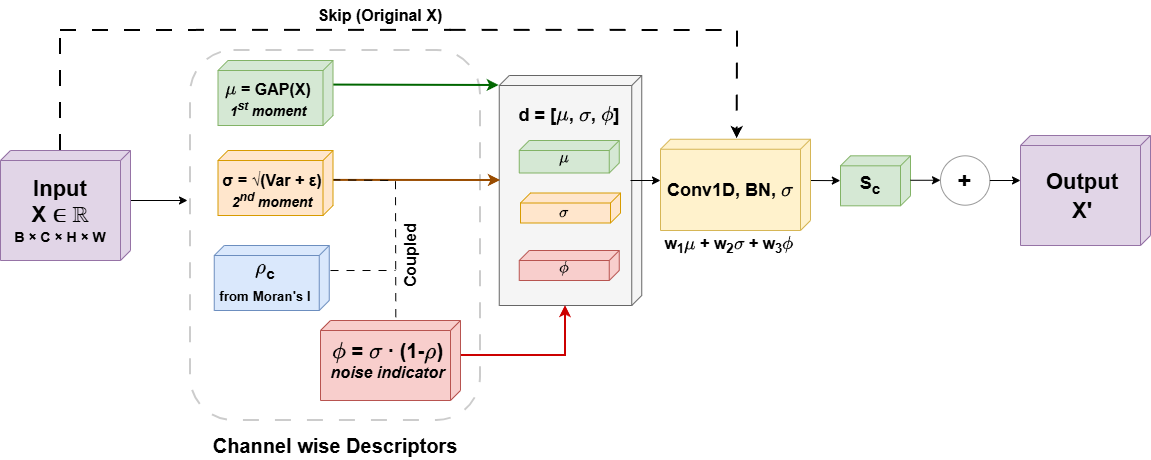
\includegraphics[width=0.7\textwidth]{ChannelExcitation.drawio (1) (2).png}
    }
    \caption{Architecture of the proposed channel excitation LACE. The noise indicator term $\phi$ takes into account the anti-correlation between $\sigma$ and $\rho$, and produces a conjunctive query that is large only when variance is high and coherence is low, which is a unique signature of spatially incoherent noise. A single weight $w_3$ directly encodes the penalization of noisy channels.}
    \label{fig:placeholder}
\end{figure}


The tendency for nearby locations within a spatial domain to exhibit greater similarity than expected by chance is formally captured by spatial autocorrelation, a concept well established since the mid-20th century in geography, ecology, and spatial econometrics. The first measure is Moran's $I$ \textbf{\cite{moran1950}} defined for $N$ observations $\{x_k\}_{k=1}^N$ with spatial adjacency weights $\{w_{kl}\}$ as:
\begin{equation}\label{eq:moran}
    I = \frac{N}{\sum_{k,l} w_{kl}} \cdot \frac{\sum_k \sum_l w_{kl}\,(x_k - \bar{x})(x_l - \bar{x})}{\sum_k (x_k - \bar{x})^2}.
\end{equation}

% Moran $I$ is the spatial analogous to the serial correlation coefficient in time series analysis and the Durbin-Watson statistic in econometrics \textbf{(citation?)}. Here, our question is a more precise version of this: \textit{are places that are close together geographically more likely to have similar values?} Positive $I$ indicates clustering (nearby values are similar), negative $I$ indicates dispersion (nearby values are dissimilar), and $I \approx -1/(N-1)$ indicates spatial randomness. \textbf{(N?)}

% The link to channel attention is direct. A convolutional feature map $\mathbf{X}_c \in \mathbb{R}^{H \times W}$ is a scalar field on a regular lattice, which is the canonical domain for spatial autocorrelation analysis. A channel that is encoding a meaningful visual feature will show positive spatial autocorrelation. Here, activations are locally coherent because the underlying image structure is spatially extended. The autocorrelation of a noisy channel is nearly zero \textbf{(nearly zero?)} since the noise, which is spatially independent, wipes out the spatial coherence created by the convolutional filter. Moran’s I measures this very difference. 
%\textbf{(I have questions about this paragraph)}

Moran's $I$ is the spatial analogue of the serial correlation coefficient in time series: it measures whether nearby observations are more similar than expected under a no-spatial-structure null. The question it formalizes is: \textit{are values at locations close together geographically more likely to be similar?} Positive $I$ indicates clustering (nearby values tend to be similar), negative $I$ indicates dispersion (nearby values tend to be dissimilar), and $I \approx -1/(N-1)$, where $N=HW$ is the number of grid cells, is the expectation under spatial randomness. The link to channel attention is direct. A convolutional feature map $\mathbf{X}_c \in \mathbb{R}^{H \times W}$ is a scalar field on a regular lattice, which is the canonical domain for spatial autocorrelation analysis. A channel that encodes a meaningful visual feature shows positive spatial autocorrelation: activations are
locally coherent because the underlying image structure is spatially extended and the convolutional filter preserves this coherence. A channel that is dominated by spatially independent noise has lag-1 autocorrelation that is small in magnitude; in expectation it is
$-1/(N-1)$, and in a finite sample it concentrates around this value with a variance that decreases as $N$ grows. Moran's $I$ measures this difference between coherent and noise-dominated channels, and the difference is what we exploit.


On a regular $H \times W$ grid, the adjacency structure must be specified. We adopt rook contiguity - horizontal and vertical neighbors only: $w_{(i,j),(i',j')} = \mathbf{1}\!\big[|i-i'| + |j-j'| = 1\big]$, where $\mathbf{1}[\cdot]$ is the indicator function. Under this binary adjacency, Moran's $I$ (Eq.~\ref{eq:moran}) reduces to the \textit{lag-1 spatial Pearson autocorrelation coefficient}, which is denoted by $\rho_c$, and computed in three steps.


\smallskip\noindent\textbf{Step 1. Centering:}
\begin{equation}\label{eq:center}
    \tilde{x}_c(i,j) = x_c(i,j) - \mu_c, \qquad \mu_c = \frac{1}{HW}\sum_{i,j} x_c(i,j).
\end{equation}

% \noindent\textbf{Step 2. Averaging neighbor cross-products:}
% \begin{align}
%     R_h &= \frac{1}{H(W{-}1)} \sum_{i=1}^{H}\sum_{j=1}^{W-1} \tilde{x}_c(i,j)\cdot\tilde{x}_c(i,j{+}1), \label{eq:rh}\\[4pt]
%     R_v &= \frac{1}{(H{-}1)W} \sum_{i=1}^{H-1}\sum_{j=1}^{W} \tilde{x}_c(i,j)\cdot\tilde{x}_c(i{+}1,j). \label{eq:rv}
% \end{align}

\noindent\textbf{Step 2. Averaging neighbor cross-products:}
\begin{alignat}{2}
    R_h &= \frac{1}{H(W{-}1)} \sum_{i=1}^{H}\sum_{j=1}^{W-1}
           \tilde{x}_c(i,j)\cdot\tilde{x}_c(i,j{+}1),
    &\quad
    R_v &= \frac{1}{(H{-}1)W} \sum_{i=1}^{H-1}\sum_{j=1}^{W}
           \tilde{x}_c(i,j)\cdot\tilde{x}_c(i{+}1,j).
    \label{eq:rhrv}
\end{alignat}

\noindent\textbf{Step 3. Normalizing to obtain Pearson correlation:}
\begin{equation}\label{eq:rho}
    \rho_c = \frac{R_h + R_v}{2\,\big(\mathrm{Var}(\mathbf{X}_c) + \epsilon\big)}, \qquad \mathrm{Var}(\mathbf{X}_c) = \frac{1}{HW}\sum_{i,j}\tilde{x}_c(i,j)^2,
\end{equation}
where $\epsilon = 10^{-5}$ ensures numerical stability. The result $\rho_c \in (-1, 1)$ measures the average correlation between each pixel and its immediate grid neighbors.

The lag-1 autocorrelation captures the dominant spatial dependence structure. The spatial coherence signal that distinguishes structured features from noise is a first-order phenomenon: it is present at the finest spatial scale and does not require higher-order or directional decomposition, as confirmed by our ablations with (a) directional decomposition ($\rho_h, \rho_v$ as separate descriptors), (b)~queen contiguity (adding diagonal neighbors), and (c)~lag-2 neighbors. Furthermore, Eq.~\ref{eq:rhrv} becomes element-wise multiplication of the feature map with its own shifted copy, a single tensor operation costing $\mathcal{O}$(HW) per channel, the same as variance. Greater lags or diagonal neighbors would necessitate extra shifting operations with declining marginal information.

The intuition behind $\rho_c$ emerges from the frequency domain, via the Wiener-Khinchin theorem \cite{wiener1930, khintchine1934}, as explained in the subsequent subsection.

\subsection{Autocorrelation as a Spectral Ratio}\label{spectral}
We first delimit what follows. The computation of $\rho_c$ in Eqs.~\ref{eq:center}--\ref{eq:rho} is a well-defined sample statistic on any finite grid and requires no stationarity assumption whatsoever. Wide-sense stationarity is invoked only for the frequency-domain reading given below, which we use as an intuition-building tool valid in the large-sample limit, and not as a claim that holds exactly on, say, a $4\times4$ grid.
For a wide-sense stationary process, the Wiener-Khinchin theorem establishes that the autocorrelation function $R(\tau)$ and the power spectral density $S(f)$ form a Fourier transform pair:
\begin{equation}\label{eq:wk}
    R(\tau) = \int_{-1/2}^{1/2} S(f)\, e^{2\pi i f \tau}\, df.
\end{equation}
At lag $\tau = 0$:
\begin{equation}\label{eq:r0}
    R(0) = \int_{-1/2}^{1/2} S(f)\, df = \text{total energy (= variance)}.
\end{equation}
At lag $\tau = 1$:
\begin{equation}\label{eq:r1}
    R(1) = \int_{-1/2}^{1/2} S(f)\, e^{2\pi i f}\, df = \int_{-1/2}^{1/2} S(f)\,\cos(2\pi f)\, df,
\end{equation}
where the imaginary part vanishes by the symmetry of $S(f)$ for real-valued signals. The weighting function $\cos(2\pi f)$ is +1 at $f = 0$ (DC/low frequency), smoothly decreasing to 0 at $f = 1/4$ (mid frequency), and $-1$ at $f = 1/2$ (Nyquist/highest frequency). Normalizing:
\begin{equation}\label{eq:rho_spectral}
    \rho = \frac{R(1)}{R(0)} = \frac{\int S(f)\cos(2\pi f)\,df}{\int S(f)\,df}.
\end{equation}

Hence, $\rho$ is the cosine-weighted average of the normalized power spectrum. It measures the proportion of total energy concentrated at low spatial frequencies relative to high spatial frequencies. Read in this way, $\rho$'s behaviour under the corruption families of interest follows from the definition rather than remaining an empirical observation. In the regime where the stationarity assumption above is reasonable:

\begin{enumerate}
    \item \textbf{Additive Gaussian noise:} White noise has a flat power spectrum, $S_n(f) = \sigma_n^2$ for all $f$, so adding it to a signal gives $S_{\text{total}}(f) = S_{\text{signal}}(f) + \sigma_n^2$. The two integrals in Eq.~\ref{eq:rho_spectral} respond to this flat term quite differently. In the denominator it contributes its full energy, $\int_{-1/2}^{1/2}\sigma_n^2\,df = \sigma_n^2$. In the numerator it is weighted by $\cos(2\pi f)$, which is positive for $f < 1/4$ and negative for $f > 1/4$; over the full band these contributions cancel, $\int_{-1/2}^{1/2}\sigma_n^2\cos(2\pi f)\,df = 0$, and on a finite grid the residual is small. The noise therefore adds unambiguously to the denominator while adding little to the numerator, and the normalized ratio $\rho$ \textbf{decreases}.

    \item \textbf{Gaussian blur:} A blur kernel with width $k$ acts as a low-pass filter with transfer function $H(f) = e^{-2\pi^2 k^2 f^2}$, so $S_{\text{blur}}(f) = |H(f)|^2 S(f)$, which suppresses high-frequency energy while preserving low-frequency energy. Since $\cos(2\pi f) > 0$ at low frequencies, the ratio in Eq.~\ref{eq:rho_spectral} shifts toward the preserved low frequencies. As a result, $\rho$ \textbf{increases}.

    \item \textbf{Contrast scaling:} For $\mathbf{Y} = a\mathbf{X}$: $S_Y(f) = a^2 S_X(f)$. Both numerator and denominator of Eq.~\ref{eq:rho_spectral} scale by $a^2$, which cancels. As a result, $\rho$ \textbf{unchanged} (a special case of the affine invariance proven in the subsequent subsection). 
\end{enumerate}


\subsection{Affine Invariance of LACE}

For any affine transformation $\mathbf{Y} = a\mathbf{X} + b$ with $a \neq 0$: $\rho_{\mathbf{Y}} = \rho_{\mathbf{X}}$. Centering eliminates the shift: $\tilde{\mathbf{Y}} = \mathbf{Y} - \mathbb{E}[\mathbf{Y}] = a\,\tilde{\mathbf{X}}$. Then:
\begin{equation}
    \rho_{\mathbf{Y}} = \frac{\mathbb{E}[\tilde{Y}_i \tilde{Y}_j]}{\mathrm{Var}(\mathbf{Y})} = \frac{a^2\,\mathbb{E}[\tilde{X}_i \tilde{X}_j]}{a^2\,\mathrm{Var}(\mathbf{X})} = \rho_{\mathbf{X}}. 
\end{equation}

Batch normalization is an affine transformation with $a = \gamma_c/\sigma_{\text{run},c}$ and $b = \beta_c - \gamma_c\frac{\mu_{\text{run},c}}{\sigma_{\text{run},c}}$, so $\rho_c$ computed on post-BN features equals $\rho_c$ computed on raw convolutional outputs. To the best of our knowledge, $\rho$ is the first channel descriptor in the attention literature that is invariant to batch normalization by construction rather than by architectural workaround.  The derivation above is exact for the idealized ratio. The implemented estimator (Eq.~\ref{eq:rho}) carries the stabilizer $\epsilon = 10^{-5}$ in its denominator, so the invariance is exact only in the limit $\epsilon \to 0$ and approximate otherwise. The approximation is tight where it matters: for a channel whose variance is on the order of the activation scale, the deviation $|\rho_{\mathbf{Y}} - \rho_{\mathbf{X}}|$ across BN scale factors $a \in [0.1, 10]$ stays below $10^{-3}$. It becomes appreciable only when $a^2\,\mathrm{Var}(\mathbf{X})$ approaches $\epsilon$, that is, for nearly-dead channels whose contribution to the gate is negligible in any case. The invariance thus holds to high precision exactly where the channel carries signal and degrades exactly where it does not. However, an important thing to note is that $\sigma_c$ and $\rho_c$ are highly anti-correlated under the Hendrycks \& Dietterich corruption benchmark: noise increases $\sigma$ while decreasing $\rho$; blur decreases $\sigma$ while increasing $\rho$. To obtain complementary information from these two descriptors, we define 

\begin{equation}\label{eq:phi}
    \phi_c = \sigma_c \cdot (1 - \rho_c).
\end{equation}
This product is large if and only if both conditions are simultaneously satisfied: variance is high ($\sigma_c$ large) and spatial coherence is low ($\rho_c$ small, hence $1 - \rho_c$ large). Neither condition alone suffices. High $\sigma$ with high $\rho$ (a structured feature) produces a small $\phi$, because of the factor $(1- \rho)$. Likewise, low $\sigma$ with low $\rho$ (a dead channel) produces a small $\phi$, because of the factor $\sigma$. The linear combination $a_c = w_{c,1}\,\mu_c + w_{c,2}\,\sigma_c + w_{c,3}\,\phi_c$ can then encode the required logic with a single sign: a negative $w_{c,3}$ penalizes channels in which high variance co-occurs with low spatial coherence. We do not claim that this interaction is otherwise unreachable. A sigmoid applied after a linear combination of $\sigma_c$ and $\rho_c$ can approximate multiplicative behaviour to some degree, but a single such unit has linear level sets in the $(\sigma_c, \rho_c)$ plane, whereas the decision boundary implied by $\phi_c$ is hyperbolic. Precomputing $\phi_c$ therefore supplies the gate with the curved feature directly, rather than requiring it to approximate the product from the two descriptors fed in separately. The preceding analysis motivates a channel attention mechanism built on three descriptors: $\mu_c$ (activation strength), $\sigma_c$ (activation spread), and $\phi_c = \sigma_c(1-\rho_c)$ (noise interaction indicator). The architecture of LACE wraps these in the simplest possible weighting scheme.

\subsubsection{Descriptor Vector.}
\begin{equation}\label{eq:desc}
    \mathbf{d}_c = [\mu_c,\; \sigma_c,\; \phi_c]^\top \in \mathbb{R}^3.
\end{equation}

\paragraph{Detached gradient.} The interaction term is detached from the computation graph before entering the gate:
\begin{equation}
\phi_c \;=\; \texttt{stop\_gradient}\!\left(\sigma_c \cdot (1-\rho_c)\right).
\label{eq:detach}
\end{equation}
We adopted this empirically as training was consistently more stable with the detachment than without it.

\subsubsection{Channel-wise Linear Combination.}

Following SRM's channel-independence principle:
$ s_c = \sigma_{\text{sig}}\!\Big(\mathrm{BN}\big(w_{c,1}\,\mu_c + w_{c,2}\,\sigma_c + w_{c,3}\,\phi_c\big)\Big),$ where $\mathbf{w}_c \in \mathbb{R}^3$ are learnable parameters specific to channel $c$, BN is one-dimensional Batch Normalization, and $\sigma_{\text{sig}}$ is the sigmoid. Implemented as \texttt{Conv1d(C, C, k=3, groups=C)} 
on $\mathbf{D} \in \mathbb{R}^{B \times C \times 3}$.

\vspace{-2.0\baselineskip}
\paragraph{Placement in the backbones.} The placement rule is the same in every backbone: LACE acts on a feature tensor produced by a $3{\times}3$ or depthwise $3{\times}3$ convolution, positioned ahead of the BN layer that would otherwise absorb its descriptors by collapsing $\mu_c$ and $\sigma_c$ to the learned constants $\beta_c$ and $|\gamma_c|$. The rule concerns that particular BN layer, not every BN in the network; the module is inserted once per block at the site identified below, and other BN layers elsewhere in the backbone are unaffected by, and irrelevant to, this choice. The three architectures, we evaluate instantiate this rule as follows. In ResNet-18, the module is inserted inside each \texttt{BasicBlock} between \texttt{bn2} and the residual addition. In MobileNetV2, the module is inserted inside each inverted-residual block on the depthwise convolution output, on the expanded ($\textit{hid}$) channels, before the $1{\times}1$ linear projection which is the canonical placement used by SE-MobileNetV3. In DenseNet-BC-100-12, the module is inserted inside each \texttt{DenseLayer} on the output of the $3{\times}3$ convolution, on the $g$ growth-rate channels, before the concatenation with the input feature map. In ResNet-50, the module is inserted inside each \texttt{Bottleneck} block on the output of \texttt{bn2} (following the $3{\times}3$ convolution \texttt{conv2}), before the $1{\times}1$ projection convolution \texttt{conv3}; LACE therefore acts on the bottleneck-width channels rather than the block's full expanded output channels. Figure \ref{fig:placeholder} summarizes the unified architecture. The steps of the proposed methodology are found in Algorithm \ref{alg:proposedalgorithm}.

\begin{algorithm}[h]
\caption{Algorithm for the proposed LACE}
\label{alg:proposedalgorithm}
\begin{algorithmic}[1]
\Require Feature map $\mathbf{X} \in \mathbb{R}^{B \times C \times H \times W}$
\Statex \textbf{Params:} $\mathbf{w} \in \mathbb{R}^{C \times 3}$,\; $\gamma, \beta \in \mathbb{R}^{C}$ \text{(BN)}
\Ensure Recalibrated $\mathbf{X}' \in \mathbb{R}^{B \times C \times H \times W}$
\For{each channel $c = 1, \ldots, C$}
    \State $\mu_c \gets \mathrm{mean}(\mathbf{X}_c)$,\;\; $\sigma_c \gets \sqrt{\mathrm{Var}(\mathbf{X}_c) + \epsilon}$
    \State $\tilde{\mathbf{X}}_c \gets \mathbf{X}_c - \mu_c$ \Comment{center activations}
    \State $R_h \gets \mathrm{mean}\!\big(\tilde{\mathbf{X}}_c^{[:,\,:\!-\!1]} \!\odot\, \tilde{\mathbf{X}}_c^{[:,\,1:]}\big)$ \Comment{horizontal cross-product}
    \State $R_v \gets \mathrm{mean}\!\big(\tilde{\mathbf{X}}_c^{[:\!-\!1,\,:]} \!\odot\, \tilde{\mathbf{X}}_c^{[1:,\,:]}\big)$ \Comment{vertical cross-product}
    \State $\rho_c \gets (R_h + R_v)\, /\, \big(2(\mathrm{Var}(\mathbf{X}_c) + \epsilon)\big)$ \Comment{lag-1 autocorrelation}
    \State $\phi_c \gets \texttt{stop\_grad}\!\big(\sigma_c \cdot (1 - \rho_c)\big)$ \Comment{noise interaction term}
    \State $s_c \gets \sigma_{\text{sig}}\!\big(\mathrm{BN}(w_{c,1}\mu_c + w_{c,2}\sigma_c + w_{c,3}\phi_c)\big)$ \Comment{channel weight}
\EndFor
\State \Return $\mathbf{s} \odot \mathbf{X}$ \Comment{recalibrate}
\end{algorithmic}
\end{algorithm}




\section{Results and Discussion} \label{results}

We evaluate the proposed channel attention against seven baselines: SE-Net~\cite{hu2018squeeze},
CBAM~\cite{woo2018cbam}, SRM~\cite{lee2020srm}, ECA-Net~\cite{wang2020eca}, FCA-Net~\cite{qin2021fcanet},
SCSA~\cite{si2022scsa}, and ELA~\cite{xu2021ela} across three backbones, namely ResNet-18, DenseNet-BC-100-12 and MobileNetV2, and three datasets, namely CIFAR-10, GTSRB and MiniImageNet. ResNet-50 on ImageNet-1k was compared against the best performing SRM~\cite{lee2020srm} and ECA~\cite{wang2020eca} only due to a constraint in computational resources. All models are trained on clean images only and evaluated on the corresponding *-C corruption benchmarks generated with the imagecorruptions library at the 15 standard Hendrycks corruption types and 5 severity levels. Mean-C accuracy is the average over all corruption types and severities. The severities are divided into 4 subcategories: Noise consists of gaussian noise, shot noise, impulse noise; Blur consists of defocus blur, glass blur, motion blur, zoom blur; Weather comprises snow, fog, frost, brightness and Digital encompasses contrast, elastic transform, pixelate and jpeg compression. The per-corruption reported accuracies are provided in details in the \href{https://github.com/KushajM/LACE-Lag-1-Autocorrelation-based-Channel-Excitation}{Github Link.}

% \paragraph{Experimental setup.} All models are trained from scratch with Stochastic Gradient Descent (SGD) (momentum 0.9, weight decay $5\times10^{-4}$, Nesterov), batch size 128, cosine learning rate schedule from 0.1, and AMP mixed precision. 

\subsection{Performance comparison}

Table~\ref{tab:performance} reports clean and Mean-C accuracy across all nine (backbone, dataset) pairs, where Mean-C is averaged over 15 corruption types across 5 severity levels on three seeds, with per-method standard deviations reported alongside the mean. LACE wins Mean-C in 9 of 9 cells without sacrificing clean accuracy, in fact clean accuracy is preserved or improved over the no-attention baseline in every single cell, with gains of up to $1.59\%$ on MobileNetV2. This demonstrates that LACE does not face the common trade-off between clean and corrupted performance.

The most substantial corruption-robustness improvements are on ResNet-18 - CIFAR-10 (Mean-C $79.87\%$ vs.\ next best $77.25\%$ by SRM, $+2.62\%$) and GTSRB ($80.80\%$ vs.\ $78.31\%$ by ECA, $+2.49\%$) and on MobileNetV2: CIFAR-10 ($78.33\%$ vs.\ $76.19\%$ by SRM, $+2.14\%$) and GTSRB ($79.02\%$ vs.\ $76.83\%$ by ELA, $+2.19\%$). On DenseNet-BC-100-12 + GTSRB the gain is $3.21\%$ Mean-C over the next best (SCSA, $74.33\%$), the largest margin across all nine cells. These gains are consistent across all 15 corruptions across 5 severity levels, not driven by outlier corruption types. 

Table~\ref{tab:performanceimagenet} reports clean and Mean-C accuracy on ImageNet-1k with the ResNet-50 backbone. We compare against SRM and ECA-Net, the closest competitors to LACE at smaller scale, each evaluated over a single seed given the compute cost of ImageNet-scale training. The estimator-reliability concern raised elsewhere (small $4{\times}4$ grids) works in LACE's favor here, since deep-stage $7{\times}7$ feature maps give $\rho$ more samples to estimate from, so this is conservative rather than favorable comparison. LACE improves clean accuracy to $77.18\%$ (vs.\ $75.73\%$, ECA-Net) and Mean-C to $44.56\%$ (vs.\ $42.84\%$, SRM), consistent with the smaller-scale trend.


% Due to a constraint in computational resources, we report the performance of each model on ImageNet-100, a 100-class subset of ImageNet-1k introduced by Tian et al. \cite{tian2020cmc} for contrastive representation learning and now widely used as a tractable proxy for full ImageNet evaluation. Clean accuracy, Mean Corruption Accuracy on ImageNet-100-C, and ImageNet-Sketch-100 accuracy are averaged over three seeds to control for run-to-run variance, with per-method standard deviations reported alongside the mean. ImageNet-Sketch-100 is constructed by intersecting ImageNet-Sketch \cite{wang2019imagenetsketch} with the 100 wordnet IDs of the CMC ImageNet-100 split. Since ImageNet-Sketch covers all 1000 ImageNet classes with approximately 50 sketches per class, this gives a test set of roughly 5000 sketches whose class label space exactly matches the training label space. No additional training is performed; models trained on the clean ImageNet-100 training images are evaluated zero-shot on the corresponding sketches. This provides one real-world distribution shift evaluation beyond the synthetic corruptions in ImageNet-100-C.

% \begin{table}[htbp]
% \centering
% \caption{Clean and mean-corruption accuracy across three datasets and three backbones. \textbf{Bold} indicates the best result per column.}
% \label{tab:performance}
% \resizebox{\textwidth}{!}{%
% \begin{tabular}{ll cc cc cc}
% \toprule
% \multirow{2}{*}{Backbone} & \multirow{2}{*}{Method}
%   & \multicolumn{2}{c}{CIFAR-10}
%   & \multicolumn{2}{c}{GTSRB}
%   & \multicolumn{2}{c}{MiniImageNet} \\
% \cmidrule(lr){3-4}\cmidrule(lr){5-6}\cmidrule(lr){7-8}
%   & & Clean & Mean-C & Clean & Mean-C & Clean & Mean-C \\
% \midrule
% \multirow{9}{*}{ResNet-18}
% & Baseline & $93.03$ & $74.46$ & $99.30$ & $76.22$ & $52.85$ & $21.82$ \\
% & SE       & $94.09$ & $74.08$ & $99.20$ & $77.81$ & $52.75$ & $23.37$ \\
% & CBAM     & $94.11$ & $72.21$ & $99.11$ & $74.53$ & $52.27$ & $22.78$ \\
% & SRM      & $94.36$ & $77.25$ & $98.52$ & $74.62$ & $\textbf{53.10}$ & $23.61$ \\
% & ECA      & $94.00$ & $74.67$ & $99.49$ & $78.31$ & $52.88$ & $22.82$ \\
% & FCA-Net  & $93.29$ & $72.53$ & $99.38$ & $77.25$ & $52.53$ & $22.60$ \\
% & SCSA     & $93.37$ & $76.06$ & $99.26$ & $73.30$ & $52.06$ & $23.15$ \\
% & ELA      & $93.33$ & $72.86$ & $99.24$ & $77.40$ & $51.86$ & $22.40$ \\
% & \textbf{Proposed} & $\textbf{94.87}$ & $\textbf{79.87}$ & $\textbf{99.89}$ & $\textbf{80.80}$ & $\underline{52.98}$ & $\textbf{24.44}$ \\
% \midrule
% \multirow{9}{*}{DenseNet-BC-100-12}
% & Baseline & $93.45$ & $68.87$ & $99.16$ & $71.59$ & $\textbf{56.72}$ & $22.84$ \\
% & SE       & $93.85$ & $70.73$ & $98.82$ & $71.78$ & $55.25$ & $23.62$ \\
% & CBAM     & $93.87$ & $71.72$ & $98.33$ & $68.79$ & $56.07$ & $23.29$ \\
% & SRM      & $93.91$ & $71.49$ & $98.35$ & $73.72$ & $50.13$ & $22.44$ \\
% & ECA      & $94.19$ & $72.80$ & $98.13$ & $71.81$ & $54.59$ & $23.90$ \\
% & FCA-Net  & $93.56$ & $71.29$ & $98.39$ & $72.84$ & $56.10$ & $23.85$ \\
% & SCSA     & $93.22$ & $70.07$ & $98.96$ & $74.33$ & $55.69$ & $23.66$ \\
% & ELA      & $94.15$ & $70.75$ & $98.84$ & $71.13$ & $53.24$ & $22.51$ \\
% & \textbf{Proposed} & $\textbf{94.98}$ & $\textbf{72.96}$ & $\textbf{99.18}$ & $\textbf{77.54}$ & $\underline{56.26}$ & $\textbf{24.48}$ \\
% \midrule
% \multirow{9}{*}{MobileNetV2}
% & Baseline & $93.56$ & $69.48$ & $\textbf{99.35}$ & $73.42$ & $49.75$ & $20.72$ \\
% & SE       & $93.73$ & $70.71$ & $99.03$ & $74.77$ & $50.53$ & $20.44$ \\
% & CBAM     & $92.38$ & $69.90$ & $98.94$ & $72.24$ & $50.27$ & $20.49$ \\
% & SRM      & $94.34$ & $76.19$ & $97.85$ & $71.43$ & $50.28$ & $21.12$ \\
% & ECA      & $94.03$ & $73.72$ & $99.18$ & $72.92$ & $49.62$ & $21.10$ \\
% & FCA-Net  & $93.38$ & $72.32$ & $99.04$ & $74.82$ & $50.32$ & $20.55$ \\
% & SCSA     & $93.18$ & $69.67$ & $98.87$ & $75.28$ & $50.92$ & $21.40$ \\
% & ELA      & $93.18$ & $70.79$ & $99.01$ & $76.83$ & $49.68$ & $21.04$ \\
% & \textbf{Proposed} & $\textbf{95.15}$ & $\textbf{78.33}$ & $\underline{99.30}$ & $\textbf{79.02}$ & $\textbf{52.26}$ & $\textbf{22.56}$ \\
% \bottomrule
% \end{tabular}}
% \end{table}

\begin{table*}[t]
\centering
\caption{Clean and mean-corruption accuracy across three datasets CIFAR-10, GTSRB and MiniImageNet and three backbones ResNet-18, DenseNet-BC-100-12 and MobileNetV2.}
\label{tab:performance}
\renewcommand{\arraystretch}{0.70}
\small
\resizebox{\textwidth}{!}{%
\begin{tabular}{ll cc cc cc}
\toprule
\multirow{2}{*}{Backbone} & \multirow{2}{*}{Method}
  & \multicolumn{2}{c}{CIFAR-10}
  & \multicolumn{2}{c}{GTSRB}
  & \multicolumn{2}{c}{MiniImageNet} \\
\cmidrule(lr){3-4}\cmidrule(lr){5-6}\cmidrule(lr){7-8}
  & & Clean & Mean-C & Clean & Mean-C & Clean & Mean-C \\
\midrule
\multirow{9}{*}{\rotatebox{90}{ResNet-18}}
& Baseline      & $93.03{\pm0.60}$ & $74.46{\pm0.97}$ & $99.30{\pm0.64}$ & $76.22{\pm0.92}$ & $52.85{\pm0.62}$ & $21.82{\pm0.95}$ \\
& SE            & $94.09{\pm0.22}$ & $74.08{\pm0.49}$ & $99.20{\pm0.41}$ & $77.81{\pm0.52}$ & $52.75{\pm0.32}$ & $23.37{\pm0.51}$ \\
& CBAM          & $94.11{\pm0.08}$ & $72.21{\pm0.61}$ & $99.11{\pm0.45}$ & $74.53{\pm0.63}$ & $52.27{\pm0.27}$ & $22.78{\pm0.62}$ \\
& SRM           & $94.36{\pm0.04}$ & $77.25{\pm0.99}$ & $98.52{\pm0.53}$ & $74.62{\pm0.88}$ & $52.48{\pm0.29}$ & $23.61{\pm0.94}$ \\
& ECA           & $94.00{\pm0.15}$ & $74.67{\pm0.32}$ & $99.49{\pm0.51}$ & $78.31{\pm0.41}$ & $52.02{\pm0.33}$ & $22.82{\pm0.37}$ \\
& FCA-Net       & $93.29{\pm0.12}$ & $72.53{\pm0.69}$ & $99.38{\pm0.48}$ & $77.25{\pm0.71}$ & $52.53{\pm0.30}$ & $22.60{\pm0.70}$ \\
& SCSA          & $93.37{\pm0.63}$ & $76.06{\pm0.87}$ & $99.26{\pm0.54}$ & $73.30{\pm0.84}$ & $52.06{\pm0.59}$ & $23.15{\pm0.86}$ \\
& ELA           & $93.33{\pm0.12}$ & $72.86{\pm0.39}$ & $99.24{\pm0.56}$ & $77.40{\pm0.45}$ & $51.86{\pm0.34}$ & $22.40{\pm0.42}$ \\
& \textbf{LACE} & $95.32{\pm0.22}$ & $\mathbf{79.87\pm0.47}$ & $99.89\pm0.38$ & $\mathbf{80.80\pm0.46}$ & $53.78{\pm0.30}$ & $\mathbf{24.44{\pm0.47}}$ \\
\midrule
\multirow{9}{*}{\rotatebox{90}{DenseNet}}
& Baseline      & $93.45{\pm0.34}$ & $68.87{\pm0.60}$ & $98.73{\pm0.38}$ & $68.27{\pm0.62}$ & $55.24{\pm0.36}$ & $22.84{\pm0.61}$ \\
& SE            & $93.85{\pm0.16}$ & $70.73{\pm0.72}$ & $98.82{\pm0.22}$ & $71.78{\pm0.68}$ & $55.25{\pm0.19}$ & $23.16{\pm0.70}$ \\
& CBAM          & $93.87{\pm0.38}$ & $71.72{\pm0.62}$ & $98.33{\pm0.41}$ & $68.79{\pm0.65}$ & $56.07{\pm0.40}$ & $23.29{\pm0.64}$ \\
& SRM           & $93.91{\pm0.16}$ & $71.49{\pm0.60}$ & $98.35{\pm0.24}$ & $73.72{\pm0.58}$ & $50.13{\pm0.20}$ & $22.44{\pm0.59}$ \\
& ECA           & $94.19{\pm0.25}$ & $72.80{\pm0.49}$ & $98.13{\pm0.25}$ & $71.81{\pm0.51}$ & $54.59{\pm0.25}$ & $23.90{\pm0.50}$ \\
& FCA-Net       & $93.56{\pm0.13}$ & $71.29{\pm0.60}$ & $98.39{\pm0.18}$ & $72.84{\pm0.64}$ & $56.10{\pm0.16}$ & $23.15{\pm0.62}$ \\
& SCSA          & $93.22{\pm0.38}$ & $70.07{\pm0.75}$ & $98.96{\pm0.42}$ & $74.33{\pm0.71}$ & $55.69{\pm0.40}$ & $23.06{\pm0.73}$ \\
& ELA           & $94.15{\pm0.27}$ & $70.75{\pm0.69}$ & $98.84{\pm0.31}$ & $71.13{\pm0.66}$ & $53.24{\pm0.29}$ & $22.51{\pm0.68}$ \\
& \textbf{LACE} & $94.98{\pm0.16}$ & $\mathbf{72.96\pm0.43}$ & $99.18\pm0.20$ & $\mathbf{77.54\pm0.44}$ & $57.56{\pm0.18}$ & $\mathbf{24.48{\pm0.44}}$ \\
\midrule
\multirow{9}{*}{\rotatebox{90}{MobileNetV2}}
& Baseline      & $92.49{\pm0.11}$ & $69.48{\pm0.14}$ & $98.78{\pm0.17}$ & $73.42{\pm0.21}$ & $49.75{\pm0.14}$ & $20.72{\pm0.18}$ \\
& SE            & $93.73{\pm0.19}$ & $70.71{\pm0.87}$ & $99.03{\pm0.41}$ & $74.77{\pm0.81}$ & $50.53{\pm0.30}$ & $20.44{\pm0.84}$ \\
& CBAM          & $92.38{\pm0.61}$ & $69.90{\pm0.68}$ & $98.94{\pm2.93}$ & $72.24{\pm0.72}$ & $50.27{\pm1.77}$ & $20.49{\pm0.70}$ \\
& SRM           & $94.34{\pm0.30}$ & $76.19{\pm0.26}$ & $97.85{\pm0.25}$ & $71.43{\pm0.32}$ & $50.28{\pm0.28}$ & $21.12{\pm0.29}$ \\
& ECA           & $94.03{\pm0.36}$ & $73.72{\pm0.60}$ & $99.18{\pm0.21}$ & $72.92{\pm0.63}$ & $49.62{\pm0.29}$ & $21.10{\pm0.62}$ \\
& FCA-Net       & $93.38{\pm0.17}$ & $72.32{\pm0.59}$ & $99.04{\pm0.48}$ & $74.82{\pm0.61}$ & $50.32{\pm0.33}$ & $20.55{\pm0.60}$ \\
& SCSA          & $93.18{\pm0.23}$ & $69.67{\pm0.55}$ & $98.87{\pm0.41}$ & $75.28{\pm0.59}$ & $50.92{\pm0.32}$ & $21.40{\pm0.57}$ \\
& ELA           & $93.18{\pm0.41}$ & $70.79{\pm1.06}$ & $99.01{\pm0.34}$ & $76.83{\pm0.98}$ & $49.68{\pm0.38}$ & $21.04{\pm1.02}$ \\
& \textbf{LACE} & $95.15{\pm0.08}$ & $\mathbf{78.33\pm0.46}$ & $99.30\pm0.12$ & $\mathbf{79.02\pm0.49}$ & $52.26{\pm0.10}$ & $\mathbf{23.48{\pm0.48}}$ \\
\bottomrule
\end{tabular}%
}
\end{table*}


% \begin{table}[t]
% \centering
% \caption{Clean, mean-corruption and ImageNet-Sketch-100 accuracy on ImageNet-100 with ResNet-50 backbone.}
% \label{tab:performance_imagenet100}
% \renewcommand{\arraystretch}{0.80}
% \small
% \resizebox{\columnwidth}{!}{%
% \begin{tabular}{l ccccccccc}
% \toprule
% Metric & Baseline & SE & CBAM & SRM & ECA & FCA-Net & SCSA & ELA & \textbf{LACE} \\
% \midrule
% Clean    & $--$ & $--$ & $--$ & $84.46\pm0.10$ & $85.12\pm0.05$ & $--$ & $--$ & $--$ & $\mathbf{85.16\pm0.07}$ \\
% Mean-C   & $--$ & $--$ & $--$ & $49.24\pm0.68$ & $48.68\pm0.72$ & $--$ & $--$ & $--$ & $\mathbf{50.65\pm0.81}$ \\
% Sketch-100 & $--$ & $--$ & $--$ & $--$ & $--$ & $--$ & $--$ & $--$ & $--$ \\
% \bottomrule
% \end{tabular}%
% }
% \end{table}

\begin{table}[t]
\centering
\caption{Clean and mean-corruption accuracy on the ImageNet-1k dataset on ResNet-50.}
\label{tab:performanceimagenet}
\renewcommand{\arraystretch}{0.70}
\small
\begin{tabular}{lccc}
\toprule
 & SRM & ECA-Net & \textbf{LACE} \\
\midrule
Clean  & $75.68$ & $75.73$ & $\mathbf{77.18}$ \\
Mean-C & $42.84$ & $41.62$ & $\mathbf{44.56}$ \\
\bottomrule
\end{tabular}
\end{table}


\subsection{Computational Efficiency}

Table~\ref{tab:cost} reports the parameter count, Multiply-Accumulate Operation (MAC) count, and single-image CPU inference latency for each method on MobileNetV2-CIFAR-10 (the smallest configuration in our sweep, where attention overhead is largest relative to the backbone cost). LACE adds 35,680 attention parameters - one of the smallest counts among methods that compete on Mean-C, well below SE/CBAM/FCA-Net (>500K) and below SCSA (>500K). Its MAC count is essentially the same as the no-attention baseline, and its CPU inference latency of 104~ms/image is among the lowest of any non-trivial method we tested.
ECA-Net achieves the lowest attention-parameter count of any method (81 parameters) at the cost of using only $\mu_c$ as a descriptor; the proposed method matches ECA's near-zero MAC overhead and CPU latency profile while adding $\rho_c$-derived spatial-coherence information that yields consistently stronger Mean-C accuracy.

\begin{table}[t]
\centering
\caption{Computational cost on MobileNetV2-CIFAR-10. Parameter and MAC counts are for the full network including attention modules. CPU Latency (CL) is the median single-image forward pass on CPU (200 runs).}
\label{tab:cost}
\renewcommand{\arraystretch}{0.70}
\begin{tabular}{l rrrr}
\toprule
Method & Total Params & Attn Params & MACs (M) & CL (ms) \\
\midrule
Baseline & 2{,}278{,}794 & 0          & 94.54  & 95 \\
SE       & 2{,}842{,}826 & 564{,}032  & 95.10  & 110 \\
CBAM     & 2{,}844{,}492 & 565{,}698  & 96.09  & 120 \\
SRM      & 2{,}307{,}338 & 28{,}544   & 94.58  & 100 \\
ECA      & 2{,}278{,}875 & 81         & 95.23  & 96 \\
FCA-Net   & 2{,}842{,}826 & 564{,}032  & 95.10  & 114 \\
SCSA     & 2{,}857{,}561 & 578{,}767  & 96.41  & 118 \\
ELA      & 2{,}350{,}154 & 71{,}360   & 95.08  & 105 \\
\textbf{LACE} & 2{,}314{,}474 & 35{,}680 & 94.56 & 100 \\
\bottomrule
\end{tabular}
\end{table}

The cost profile reflects the design. The proposed mechanism LACE adds three learnable scalars per channel ($w_{c,1}, w_{c,2}, w_{c,3}$) plus the BN parameters of the 1D BN layer. There is no FC bottleneck (which SE/FCA-Net pay $2C^2/r$ for) and no spatial convolution (which CBAM, SCSA, and ELA pay extra MACs for). The dominant cost in the forward pass is the lag-1 cross-product computation in Eq.~\ref{eq:rhrv}, which is two element-wise products of the centered feature map with itself shifted by one, an operation that
modern deep learning frameworks fuse efficiently.

\subsection{Ablation Study}
\label{sec:ablation}

We isolate the contribution of each design choice in our proposed method through a systematic ablation on MobileNetV2-GTSRB. We sweep two design axes holding the other fixed: (A)~the spatial definition of $\rho$ (adjacency and lag), and (B)~the descriptor composition entering the gate. The pivot variant is the proposed Rook lag-1 with descriptor $[\mu, \sigma, \phi]$. Table~\ref{tab:ablation} reports clean accuracy, Mean-C accuracy, and the four corruption-category means.

% \begin{table}[t]
% \centering
% \caption{Ablation on MobileNetV2-GTSRB. Spatial group fixes descriptor $=[\mu,\sigma,\phi]$; descriptor group fixes spatial mode = rook lag-1. The pivot configuration (proposed) combines rook lag-1 with $[\mu,\sigma,\phi]$ and is shown in the
% last row. \textbf{Bold} = best per column.}
% \label{tab:ablation}
% \resizebox{\textwidth}{!}{%
% \begin{tabular}{ll rrrrrr}
% \toprule
% Group & Variant & Clean & Mean-C & Noise & Blur & Weather & Digital \\
% \midrule
% \multirow{4}{*}{\textbf{(A) Spatial}}
% & Queen lag-1                & $99.26\pm0.47$ & $73.72\pm1.18$ & $67.80\pm1.15$ & $74.84\pm1.12$ & $68.51\pm1.19$ & $80.95\pm1.14$ \\
% & Rook lag-2                 & $98.80\pm0.48$ & $76.52\pm1.16$ & $73.07\pm1.13$ & $77.38\pm1.10$ & $70.40\pm1.17$ & $82.84\pm1.13$ \\
% & Directional ($\rho_h, \rho_v$) & $99.01\pm0.46$ & $78.43\pm1.14$ & $75.38\pm1.12$ & $78.08\pm1.09$ & $72.60\pm1.15$ & $84.45\pm1.11$ \\
% \midrule
% \multirow{3}{*}{\textbf{(B) Descriptor}}
% & $[\mu, \sigma]$            & $98.73\pm0.49$ & $71.43\pm1.00$ & $74.63\pm1.13$ & $78.14\pm1.10$ & $72.44\pm1.16$ & $84.46\pm1.12$ \\
% & $[\mu, \sigma, \rho]$      & $98.90\pm0.48$ & $74.47\pm1.00$ & $75.64\pm1.14$ & $76.86\pm1.11$ & $70.44\pm1.18$ & $84.73\pm1.13$ \\
% & $[\mu, \sigma, \rho, \phi]$ & $99.13\pm0.46$ & $78.22\pm0.96$ & $73.30\pm1.12$ & $76.65\pm1.10$ & $71.75\pm1.17$ & $84.09\pm1.11$ \\
% \midrule
% \textbf{Proposed}
% & Rook lag-1, $[\mu, \sigma, \phi]$ & $\textbf{99.30}\pm0.12$ & $\textbf{79.70}\pm0.76$ & $\textbf{78.56}\pm0.71$ & $\textbf{79.02}\pm0.79$ & $\textbf{72.82}\pm0.74$ & $\textbf{85.98}\pm0.72$ \\
% \bottomrule
% \end{tabular}}
% \end{table}

\begin{table}[h]
\centering
\caption{Ablation on the MobileNetV2-GTSRB combination. Spatial group fixes descriptor $=[\mu,\sigma,\phi]$; descriptor group fixes spatial mode = rook lag-1. The pivot configuration (LACE) combines rook lag-1 with $[\mu,\sigma,\phi]$ and is shown in the last row.}
\label{tab:ablation}
\renewcommand{\arraystretch}{0.70}
\resizebox{\columnwidth}{!}{%
\begin{tabular}{ll rrrrrr}
\toprule
Group & Variant & Clean & Mean-C & Noise & Blur & Weather & Digital \\
\midrule
\multirow{4}{*}{\textbf{(A) Spatial}}
& Queen lag-1                     & $99.26$ & $73.72$ & $67.80$ & $74.84$ & $68.51$ & $80.95$ \\
& Rook lag-2                      & $98.80$ & $76.52$ & $73.07$ & $77.38$ & $70.40$ & $82.84$ \\
& Directional ($\rho_h, \rho_v$)  & $99.01$ & $78.43$ & $75.38$ & $78.08$ & $72.60$ & $84.45$ \\
\midrule
\multirow{3}{*}{\textbf{(B) Descriptor}}
& $[\mu, \sigma]$                  & $98.73$ & $71.43$ & $70.63$ & $71.14$ & $68.44$ & $74.46$ \\
& $[\mu, \sigma, \rho]$            & $98.90$ & $74.47$ & $75.64$ & $71.86$ & $72.44$ & $76.73$ \\
& $[\mu, \sigma, \rho, \phi]$      & $99.13$ & $78.22$ & $75.30$ & $76.65$ & $71.75$ & $84.09$ \\
\midrule
\textbf{LACE}
& Rook lag-1, $[\mu, \sigma, \phi]$ & $\textbf{99.30}$ & $\textbf{79.70}$ & $\textbf{78.56}$ & $\textbf{79.02}$ & $\textbf{72.82}$ & $\textbf{85.98}$ \\
\bottomrule
\end{tabular}%
}
\end{table}

\paragraph{(A) Spatial structure.} The proposed rook lag-1 (last row) outperforms all three alternatives on Mean-C. Queen contiguity, which adds the four diagonal neighbors, performs \emph{worst} of the four spatial choices despite using strictly more information, losing 5.98\% Mean-C versus rook lag-1. We treat this as an information-versus-statistical-reliability trade-off: at the spatial scale of MobileNetV2 feature maps, adding diagonals roughly doubles the number of cross-product terms contributing to the autocorrelation estimate, and at small spatial sizes (the deepest stages reach $4\times4$ on small-image backbones) this introduces estimator variance that the gate then has to filter out. Lag-2 also underperforms by a smaller margin, which is consistent with the dominant spatial dependence being first-order. Directional decomposition ($\rho_h$ and $\rho_v$ as separate descriptors) performs reasonably but adds 7{,}136 extra parameters per attention block for no measurable Mean-C gain.

\paragraph{(B) Descriptor composition.} 

First, $[\mu, \sigma]$ alone (B1) is, in essence, an SRM-style descriptor: marginal statistics combined channel-wise. The proposed descriptor improves on it by 8.27\% which is consistent with the run-to-run Mean-C standard deviation, we cited earlier for this benchmark. The cross-backbone evidence in Table~\ref{tab:performance}, where the proposed attention beats SRM by larger margins on most cells, provides a strong support for the contribution of $\rho$. Second, replacing $\phi$ with raw $\rho$ (B2 vs. proposed) loses 5.23\% Mean-C. The conjunctive multiplicative form of $\phi$ matters: a linear-then-sigmoid gate fed $\sigma_c$ and $\rho_c$ separately has linear level sets and can only approximate the hyperbolic boundary that $\phi$ supplies directly.

\subsection{Visualizations}\label{Visualization}

% We complement the quantitative results with three visualizations, each on the (backbone, dataset) cell that best exposes what the visualization is meant to show: t-SNE on DenseNet-BC-100-12 + GTSRB because the 43 traffic-sign classes give a richer cluster structure than CIFAR-10's 10 classes; confusion matrices on ResNet-18 + CIFAR-10 because 10 classes are readable in a confusion grid; and GradCAM on DenseNet-BC-100-12 + GTSRB because the traffic-sign content makes the saliency interpretable. All three use Gaussian noise at severity 3 as the corruption.

\paragraph{Feature-space separability under corruption.}
Figure~\ref{fig:tsne} shows two-dimensional t-SNE projections of the penultimate-layer features for 2{,}000 corrupted test images, comparing the no-attention baseline (left) with the proposed module LACE (right).
Colors indicate the 43 GTSRB classes. Both models classify above chance under sev-3 Gaussian noise, but LACE retains more class structure: peripheral clusters are tighter, inter-class mixing in the central region is reduced, and several classes that are absorbed into
the central blob in the baseline emerge as distinct clusters under LACE. The plot is consistent with the quantitative gap on this cell: baseline 68.27\% Mean-C versus LACE 77.54\% (Table~\ref{tab:performance}).
 
\begin{figure}[h]
\centering
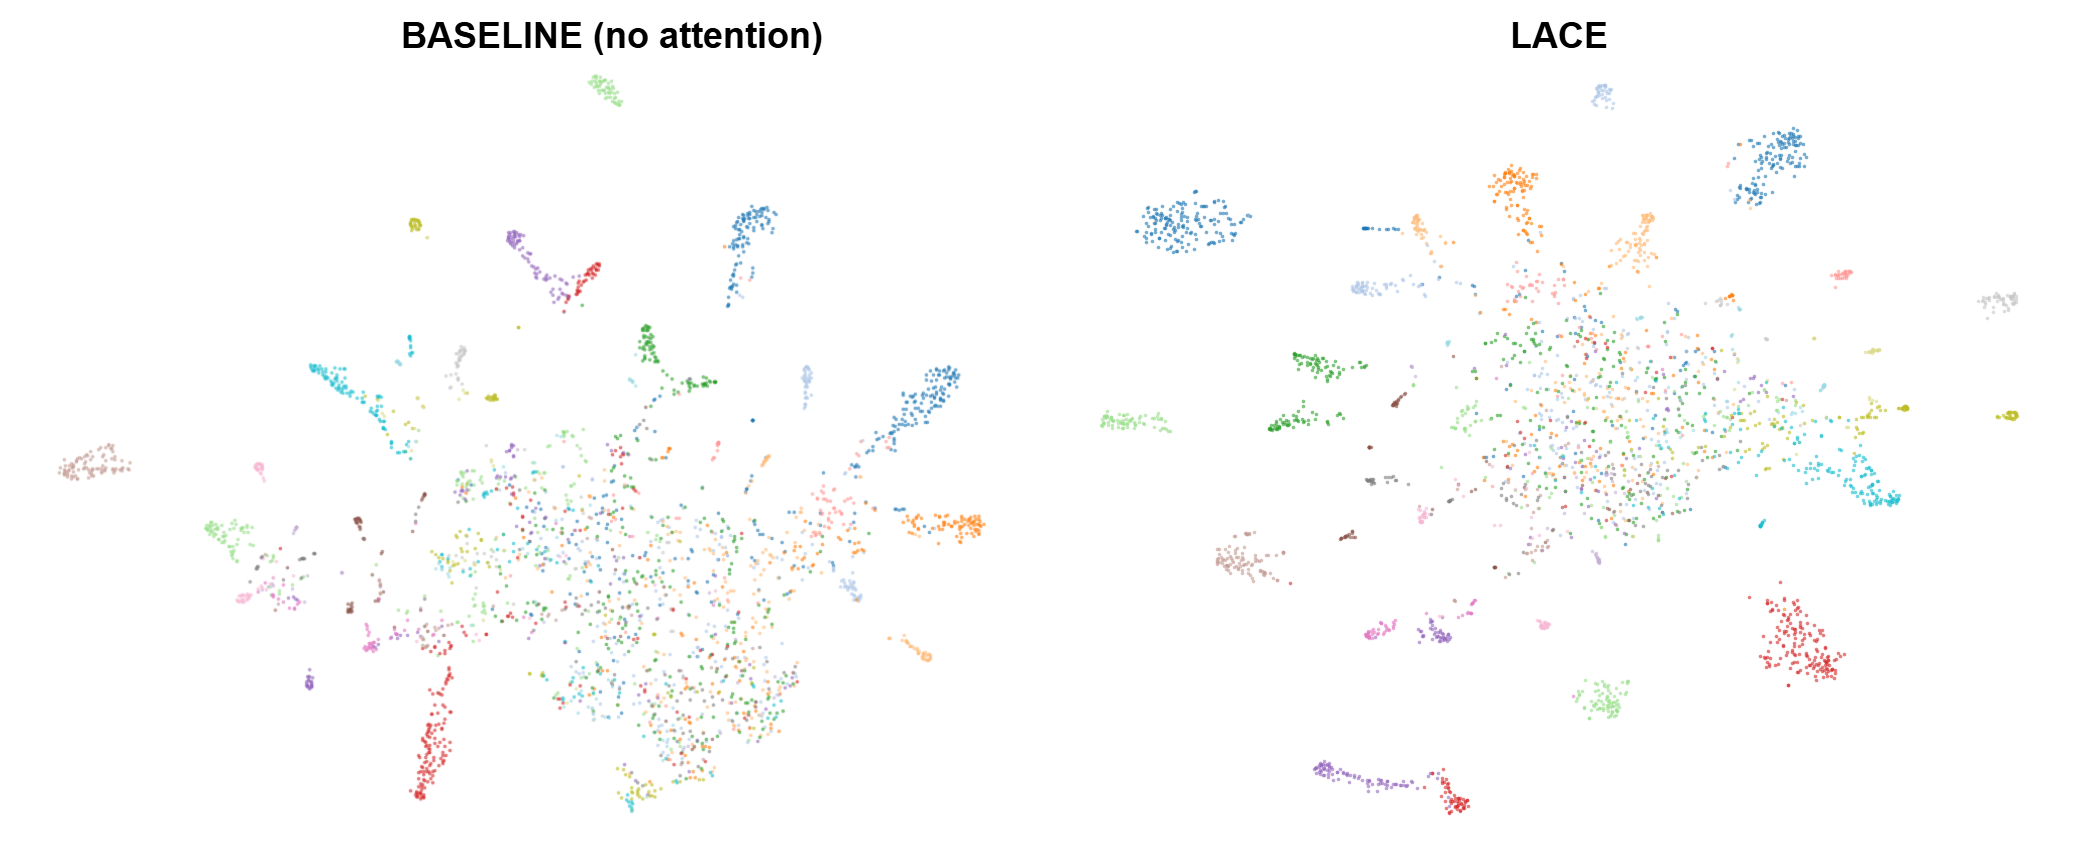
\includegraphics[width=0.7\linewidth]{LACEt-SNE.drawio (1).png}
% \hfill
% \includegraphics[width=0.48\linewidth]{tsne_proposed.png}
\caption{t-SNE projection of penultimate-layer features on GTSRB under Gaussian noise at severity 3 with DenseNet-BC-100-12. \textbf{Left}: baseline. \textbf{Right}: LACE. Colors indicate the 43 GTSRB classes. LACE preserves more inter-class separation under corruption.}
\label{fig:tsne}
\end{figure}

\paragraph{Confusion patterns under corruption.}
Figure~\ref{fig:cm} shows row-normalized confusion matrices on CIFAR-10-C with Gaussian noise at severity 3, using ResNet-18. Diagonal entries are per-class recall: a darker diagonal means more corrupted samples are
classified into the correct class. LACE's diagonal is visibly cleaner, with off-diagonal mass substantially reduced compared with the baseline, particularly among the animal classes (cat, dog, frog and bird), where the baseline systematically routes corrupted samples between visually similar categories.
 
\begin{figure}[h]
\centering
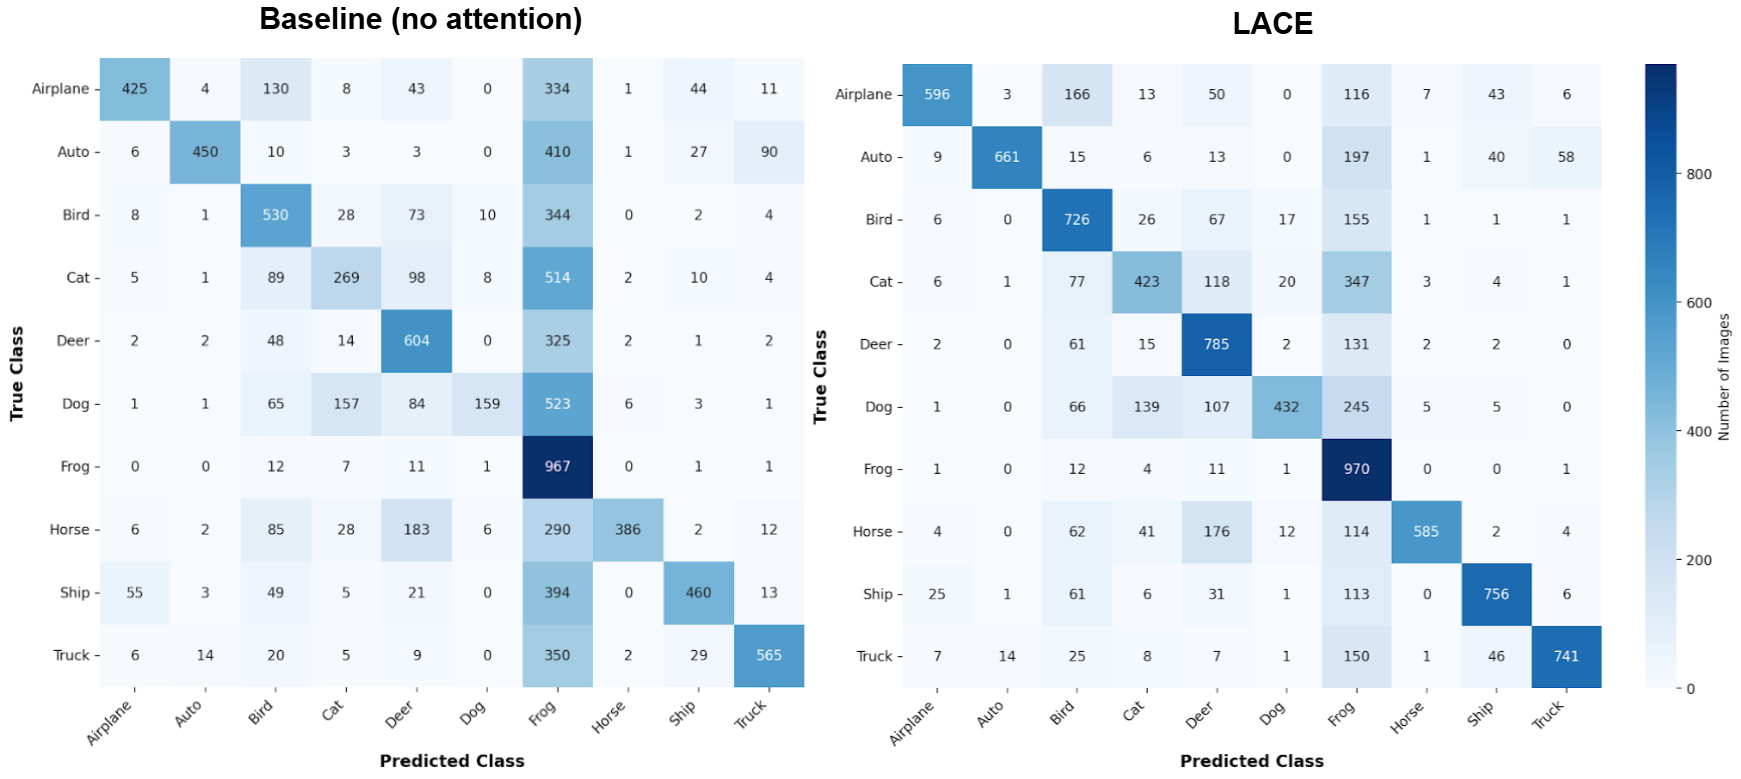
\includegraphics[width=0.7\linewidth]{LACEConfusionMatrix.drawio (1).png}
% \hfill
% \includegraphics[width=0.48\linewidth]{cm_proposed_cifar10.png}
\caption{Row-normalized confusion matrices on CIFAR-10 under Gaussian noise at severity 3 with ResNet-18. \textbf{Left}: baseline.
\textbf{Right}: LACE. LACE produces a cleaner diagonal and weaker off-diagonal confusions among visually similar class pairs.}
\label{fig:cm}
\end{figure}

% \paragraph{Where the network attends.}
% Figure~\ref{fig:gradcam} shows GradCAM saliency maps on four GTSRB classes that illustrate where LACE differs from the baseline qualitatively: cls 14 (stop sign), cls 17 (no-entry), cls 18 (general caution triangle), and cls 25 (road work triangle). For each class we show the corrupted input and the GradCAM overlay for both methods.
% Under Gaussian noise at severity 3, the baseline's attention diffuses beyond the sign boundary (visible on the stop sign and the no-entry disc) and concentrates inside flat regions of triangles instead of the discriminative apex and edges. LACE's attention stays better localized to the sign content and tracks the structural features relevant to class identity, the triangular outline rather than the interior, the disc boundary rather than ambient pixels.
 
% \begin{figure}[h]
% \centering
% \includegraphics[width=0.6\linewidth]{LACEGradCAM1.drawio (1).png}
% \caption{GradCAM saliency on four GTSRB classes under Gaussian noise at severity 3, using DenseNet-BC-100-12. \textbf{Top row}: corrupted inputs for cls 14 (stop sign), cls 17 (no-entry), cls 18 (general caution), cls 25 (road work). \textbf{Middle row}: baseline overlays.
% \textbf{Bottom row}: LACE overlays. LACE's attention stays better localized to discriminative sign content under corruption.}
% \label{fig:gradcam}
% \end{figure}


\section{Conclusion}\label{conclusion}

We argued that channel attention modules have been gating on the wrong quantity. Mean, standard deviation, and maximum all throw away spatial arrangement, and two of them collapse to BN parameters. The lag-1 spatial Pearson autocorrelation $\rho_c$ keeps the spatial information
and survives BN's affine transform, and combining it with $\sigma_c$ into the conjunctive term $\phi_c = \sigma_c(1-\rho_c)$ gives a descriptor that fires specifically on the high-variance, low-coherence signature of incoherent noise. The full descriptor $[\mu_c, \sigma_c, \phi_c]$ goes into a channel-wise linear gate with three learnable
weights per channel and adds essentially no cost over global average pooling. Across nine (backbone, dataset) configurations the module gives the best mean-corruption accuracy on all and matches clean accuracy throughout, as demonstrated in our Table~\ref{tab:performance}.
 
There are three limitations worth flagging. First, $\rho_c$ is a statistical estimate from $HW$ samples per channel, and on the deep stages of small-image backbones, where the feature map is down to $4\!\times\!4$ on CIFAR-10 ResNet-18, that estimate is noisy. The gate's learned $w$ partially absorbs this, but the small-grid regime
is the clear weak spot of the design and is also where the class-count effect we see on MiniImageNet starts to matter. Second, while $\rho_c$ is BN-invariant to within the stabilizer, $\mu_c$ and $\sigma_c$ in the descriptor vector are not: when the module is placed after a BN layer, they read the BN parameters $\beta_c$ and $|\gamma_c|$. We retain them only because in our canonical placement (after a depthwise or $3\times3$ conv, ahead of the BN that would otherwise absorb them) they read genuine activation statistics. Furthermore, LACE underperforms on brightness as compared to SRM because the affine-invariance property, which is usually a strength, means that $\rho$ is unchanged by global intensity scaling thereby providing no signal that would let the gate respond to brightness shifts. Similarly, for weather corruptions like snow that introduce structured occlusions $\rho$ misreads the corruption pattern as legitimate spatial coherence, since snow patches are themselves spatially correlated. 

Three future extensions are suggested. First is extending the experimentation to a larger dataset like the ImageNet-1k dataset, with more computational resources. The next is to swap the attention-head BN for Group Normalization, which makes the gate itself BN-independent and complements the BN-invariance of $\rho_c$. Furthermore, one could also try replacing the rook lag-1 adjacency with a learned or multi-scale weighting: the difficulty there is keeping the estimator variance under control, since adding more spatial terms is what hurt us in the queen-contiguity ablation. 

\section{Acknowledgements}

We would like to thank the CMATER Lab, Jadavpur University, Kolkata, India for giving us the platform to conduct this research.


% From 2009, the proceedings of BMVC (the British Machine Vision
% Conference) will be published only in electronic form.  This document
% illustrates the required paper format, and includes guidelines on
% preparation of submissions.  Papers which fail to adhere to these
% requirements may be rejected at any stage in the review process.

% \LaTeX\ users should use this template in order to prepare their paper.
% Users of other packages should emulate the style and layout of this
% example.  Note that best results will be achieved using {\tt pdflatex},
% which is available in most modern distributions.

% \subsection{Paper length}
% Papers for phase-one review must be 14~pages in length, {\bf only} {\em excluding} the bibliography.
% References and any appendices are unlimited.


% {\bf Papers which are
% clearly overlength will not be reviewed}.  This includes papers where the
% margins and formatting are deemed to have been significantly altered from
% those laid down by this style guide.

% The bibliography should begin immediately after the paper text.  It may
% be of any length, within reason.  It should {\em not} include
% annotations, figures, or any other paraphernalia intended to subvert the
% paper length requirement.

% \begin{figure}
% \begin{tabular}{ccc}
% \bmvaHangBox{\fbox{\parbox{2.7cm}{~\\[2.8mm]
% \rule{0pt}{1ex}\hspace{2.24mm}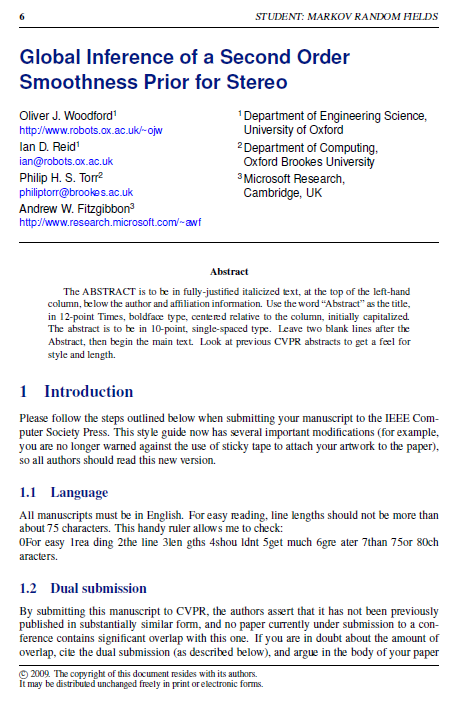
\includegraphics[width=2.33cm]{images/eg1_largeprint.png}\\[-0.1pt]}}}&
% \bmvaHangBox{\fbox{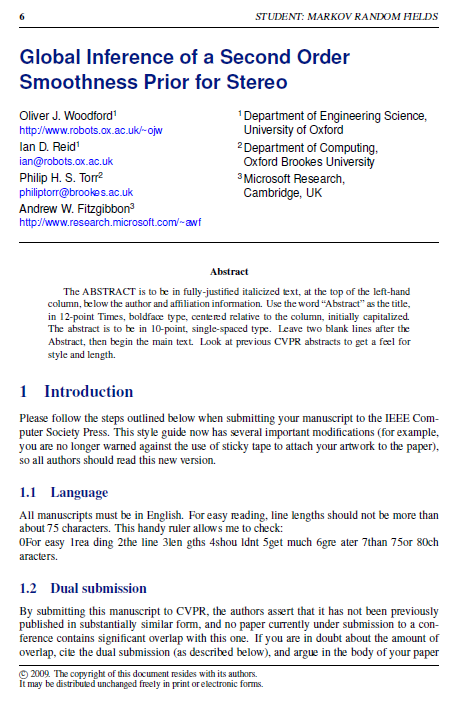
\includegraphics[width=2.8cm]{images/eg1_largeprint.png}}}&
% \bmvaHangBox{\fbox{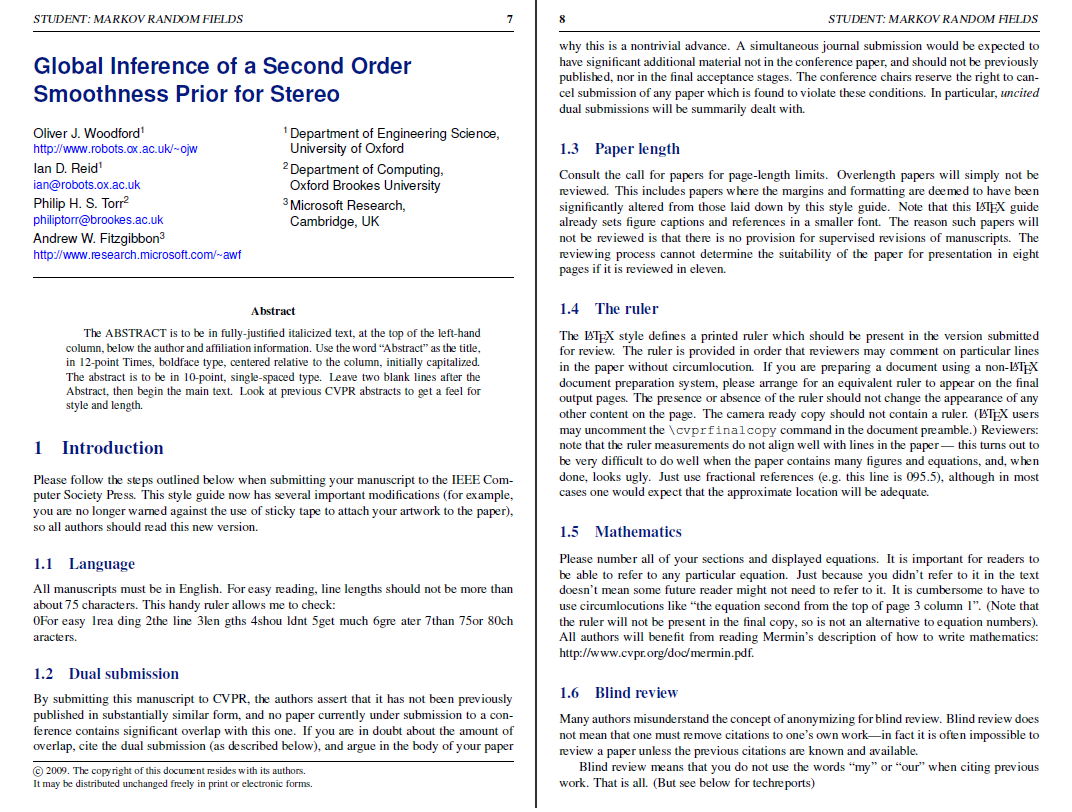
\includegraphics[width=5.6cm]{images/eg1_2up.png}}}\\
% (a)&(b)&(c)
% \end{tabular}
% \caption{It is often a good idea for the first figure to attempt to
% encapsulate the article, complementing the abstract.  This figure illustrates
% the various print and on-screen layouts for which this paper format has
% been optimized: (a) traditional BMVC print format; (b) on-screen
% single-column format, or large-print paper; (c) full-screen two column, or
% 2-up printing. }
% \label{fig:teaser}
% \end{figure}

% \subsection{Dual submission}
% By submitting this manuscript to BMVC, the authors assert that it has not
% been previously published in substantially similar form, and no paper
% currently under submission to a conference contains significant overlap
% with this one.  If you are in doubt about the amount of overlap, cite the
% dual submission (as described below), and argue in the body of your paper
% why this is a nontrivial advance.  A simultaneous journal submission would
% be expected to have significant additional material not in the conference
% paper, and should not be previously published, nor in the final acceptance
% stages. The conference chairs reserve the right to cancel
% submission of any paper which is found to violate these conditions.  In
% particular, {\em uncited} dual submissions will be summarily dealt with.

% \subsection{Anonymity and blind review}
% BMVC operates a double-blind review process.  Your review submission {\bf
% must not identify you as the author}.  This means, in particular, that the
% author list should be replaced by the words ``BMVC {\em YYYY} Submission \#
% {\em NNN}'', where the italics are to indicate the year and the submission
% number.  The provided \LaTeX\ command \verb'\bmvcreviewcopy' does this
% automatically.  In addition, acknowledgements should not be included in the
% review copy.

% Many authors misunderstand the concept of anonymizing for blind
% review.  Blind review {\bf does not mean that one must remove
% citations to one's own work}---in fact it is often impossible to
% review a paper unless the previous citations are known and
% available.

% Blind review means that you do not use the words ``my'' or ``our''
% when citing previous work.  That is all.  (But see below for
% techreports)

% Saying ``this builds on the work of Lucy Smith [1]'' does not say
% that you are Lucy Smith, it says that you are building on her
% work.  If you are Smith and Jones, do not say ``as we show in
% [7]'', say ``as Smith and Jones show in [7]'' and at the end of the
% paper, include reference 7 as you would any other cited work.

% An example of a bad paper:
% \begin{quote}
% \begin{center}
%     An analysis of the frobnicatable foo filter.
% \end{center}

%    In this paper we present a performance analysis of our
%    previous paper [1], and show it to be inferior to all
%    previously known methods.  Why the previous paper was
%    accepted without this analysis is beyond me.
%    [1] Removed for blind review
% \end{quote}


% An example of an excellent paper:

% \begin{quote}
% \begin{center}
%      An analysis of the frobnicatable foo filter.
% \end{center}

%    In this paper we present a performance analysis of the
%    paper of Smith \etal [1], and show it to be inferior to
%    all previously known methods.  Why the previous paper
%    was accepted without this analysis is beyond me.

%    [1] Smith, L and Jones, C. ``The frobnicatable foo
%    filter, a fundamental contribution to human knowledge''.
%    Nature 381(12), 1-213.
% \end{quote}

% If you are making a submission to another conference at the same time,
% which covers similar or overlapping material, you will almost certainly
% need to refer to that submission in order to explain the differences,
% just as you would if you or others had previously published related
% work.  In such cases, include the anonymized parallel
% submission~\cite{Authors06} as additional material and cite it as
% \begin{quote}
% [1] Authors. ``The frobnicatable foo filter'', ECCV 2006 Submission ID 324,
% Supplied as additional material {\tt eccv06.pdf}.
% \end{quote}

% Finally, you may feel you need to tell the reader that more details can be
% found elsewhere, and refer them to a technical report.  For conference
% submissions, the paper must stand on its own, and not {\em require} the
% reviewer to go to a techreport for further details.  Thus, you may say in
% the body of the paper ``further details may be found
% in~\cite{Authors06b}''.  Then submit the techreport as additional material.
% Again, you may not assume the reviewers will read this material.

% Sometimes your paper is about a problem which you tested using a tool which
% is widely known to be restricted to a single institution.  For example,
% let's say it's 1969, you have solved a key problem on the Apollo lander,
% and you believe that the ICLL'70 audience would like to hear about your
% solution.  The work is a development of your celebrated 1968 paper entitled
% ``Zero-g frobnication: How being the only people in the world with access to
% the Apollo lander source code makes us a wow at parties'', by Zeus \etal.

% You can handle this paper like any other.  Don't write ``We show how to
% improve our previous work [Anonymous, 1968].  This time we tested the
% algorithm on a lunar lander [name of lander removed for blind review]''.
% That would be silly, and would immediately identify the authors. Instead
% write the following:
% \begin{quotation}
% \noindent
%    We describe a system for zero-g frobnication.  This
%    system is new because it handles the following cases:
%    A, B.  Previous systems [Zeus et al. 1968] didn't
%    handle case B properly.  Ours handles it by including
%    a foo term in the bar integral.

%    ...

%    The proposed system was integrated with the Apollo
%    lunar lander, and went all the way to the moon, don't
%    you know.  It displayed the following behaviours
%    which show how well we solved cases A and B: ...
% \end{quotation}
% As you can see, the above text follows standard scientific convention,
% reads better than the first version, and does not explicitly name you as
% the authors.  A reviewer might think it likely that the new paper was
% written by Zeus \etal, but cannot make any decision based on that guess.
% He or she would have to be sure that no other authors could have been
% contracted to solve problem B.

% FAQ: Are acknowledgements OK?  No.  Leave them for the final copy.

% \subsection{Citations}
% When citing a multi-author paper, you may save space by using ``{\em et
% alia}'', shortened to ``\etal'' (not ``{\em et.\ al.}'' as ``{\em et}'' is
% a complete word.)  The provided \verb'\etal' macro is a useful {\em aide
% memoire} in this regard.  However, use it only when there are three or more
% authors.  Thus, the following is correct: `` Frobnication has been trendy
% lately.  It was introduced by Alpher~\cite{Alpher02}, and subsequently
% developed by Alpher and Fotheringham-Smythe~\cite{Alpher03}, and Alpher
% \etal~\cite{Alpher04}.''

% This is incorrect: ``... subsequently developed by Alpher \etal~\cite{Alpher03} ...''
% because reference~\cite{Alpher03} has just two authors.  If you use the
% \verb'\etal' macro, then you need not worry about double periods
% when used at the end of a sentence as in Alpher \etal.

% %For this citation style, keep multiple citations in numerical (not
% %chronological) order, so prefer
% We use {\tt natbib}, so citations in random order are nicely sorted:
%  \cite{Alpher03,Alpher02,Authors06b,Authors06}.  However, we don't use the
% compress option, as we want each reference to have its own hyperlink and
% popup window.

% %-------------------------------------------------------------------------
% \subsection{Footnotes}

% Please use footnotes\footnote {This is what a footnote looks like.  It
% often distracts the reader from the main flow of the argument.} sparingly.
% Indeed, try to avoid footnotes altogether and include necessary peripheral
% observations in
% the text (within parentheses, if you prefer, as in this sentence).  If you
% wish to use a footnote, place it at the bottom of the column on the page on
% which it is referenced. Use Times 8-point type, single-spaced.


% \begin{figure*}
% \begin{center}
% \fbox{\rule{0pt}{2in} \rule{.9\linewidth}{0pt}}
% \end{center}
%    \caption{Example of a short caption, which should be centered.}
% \label{fig:short}
% \end{figure*}

% %-------------------------------------------------------------------------
% \subsection{The ruler}
% The \LaTeX\ style defines a printed ruler which should be present in the
% version submitted for review.  The ruler is provided in order that
% reviewers may comment on particular lines in the paper without
% circumlocution.  If you are preparing a document using a non-\LaTeX\
% document preparation system, please arrange for an equivalent ruler to
% appear on the final output pages.  The presence or absence of the ruler
% should not change the appearance of any other content on the page.  The
% camera ready copy should not contain a ruler. (\LaTeX\ users may remove
% the \verb'[review]' option from the \verb'\documentclass' statement.)
% Reviewers: note that the ruler measurements do not align well with lines
% in the paper --- this turns out to be very difficult to do well when the
% paper contains many figures and equations, and, when done, looks ugly.
% Just use fractional references (e.g.\ this line is $210.5$), although in
% most cases one would expect that the approximate location ($210$ in the
% previous example) will be adequate.


% \begin{table}
% \begin{center}
% \begin{tabular}{|l|c|}
% \hline
% Method & Frobnability \\
% \hline\hline
% Theirs & Frumpy \\
% Yours & Frobbly \\
% Ours & Makes one's heart Frob\\
% \hline
% \end{tabular}
% \end{center}
% \caption{Results.   Ours is better.}
% \end{table}

% \subsection{Mathematics}

% Please number all of your sections and displayed equations.  It is
% important for readers to be able to refer to any particular equation.  Just
% because you didn't refer to it in the text doesn't mean some future reader
% might not need to refer to it.  It is cumbersome to have to use
% circumlocutions like ``the equation second from the top of page 3 column
% 1''.  (Note that the ruler will not be present in the final copy, so is not
% an alternative to equation numbers).  All authors will benefit from reading
% Mermin's description~\cite{Mermin89} of how to write mathematics.


% %-------------------------------------------------------------------------
% \subsection{References}

% List and number all bibliographical references in 9-point Times,
% single-spaced, at the end of your paper. When referenced in the text,
% enclose the citation number in square brackets, for
% example~\cite{Authors06}.  Where appropriate, include the name(s) of
% editors of referenced books.


% %------------------------------------------------------------------------
% \subsection{Color}

% Color is valuable, and will be visible to readers of the electronic copy.
% However ensure that, when printed on a monochrome printer, no important
% information is lost by the conversion to grayscale.

\bibliography{egbib}
\end{document}
